\documentclass[twoside]{book}

% Packages required by doxygen
\usepackage{fixltx2e}
\usepackage{calc}
\usepackage{doxygen}
\usepackage[export]{adjustbox} % also loads graphicx
\usepackage{graphicx}
\usepackage[utf8]{inputenc}
\usepackage{makeidx}
\usepackage{multicol}
\usepackage{multirow}
\PassOptionsToPackage{warn}{textcomp}
\usepackage{textcomp}
\usepackage[nointegrals]{wasysym}
\usepackage[table]{xcolor}

% Font selection
\usepackage[T1]{fontenc}
\usepackage[scaled=.90]{helvet}
\usepackage{courier}
\usepackage{amssymb}
\usepackage{sectsty}
\renewcommand{\familydefault}{\sfdefault}
\allsectionsfont{%
  \fontseries{bc}\selectfont%
  \color{darkgray}%
}
\renewcommand{\DoxyLabelFont}{%
  \fontseries{bc}\selectfont%
  \color{darkgray}%
}
\newcommand{\+}{\discretionary{\mbox{\scriptsize$\hookleftarrow$}}{}{}}

% Page & text layout
\usepackage{geometry}
\geometry{%
  a4paper,%
  top=2.5cm,%
  bottom=2.5cm,%
  left=2.5cm,%
  right=2.5cm%
}
\tolerance=750
\hfuzz=15pt
\hbadness=750
\setlength{\emergencystretch}{15pt}
\setlength{\parindent}{0cm}
\setlength{\parskip}{3ex plus 2ex minus 2ex}
\makeatletter
\renewcommand{\paragraph}{%
  \@startsection{paragraph}{4}{0ex}{-1.0ex}{1.0ex}{%
    \normalfont\normalsize\bfseries\SS@parafont%
  }%
}
\renewcommand{\subparagraph}{%
  \@startsection{subparagraph}{5}{0ex}{-1.0ex}{1.0ex}{%
    \normalfont\normalsize\bfseries\SS@subparafont%
  }%
}
\makeatother

% Headers & footers
\usepackage{fancyhdr}
\pagestyle{fancyplain}
\fancyhead[LE]{\fancyplain{}{\bfseries\thepage}}
\fancyhead[CE]{\fancyplain{}{}}
\fancyhead[RE]{\fancyplain{}{\bfseries\leftmark}}
\fancyhead[LO]{\fancyplain{}{\bfseries\rightmark}}
\fancyhead[CO]{\fancyplain{}{}}
\fancyhead[RO]{\fancyplain{}{\bfseries\thepage}}
\fancyfoot[LE]{\fancyplain{}{}}
\fancyfoot[CE]{\fancyplain{}{}}
\fancyfoot[RE]{\fancyplain{}{\bfseries\scriptsize Generated by Doxygen }}
\fancyfoot[LO]{\fancyplain{}{\bfseries\scriptsize Generated by Doxygen }}
\fancyfoot[CO]{\fancyplain{}{}}
\fancyfoot[RO]{\fancyplain{}{}}
\renewcommand{\footrulewidth}{0.4pt}
\renewcommand{\chaptermark}[1]{%
  \markboth{#1}{}%
}
\renewcommand{\sectionmark}[1]{%
  \markright{\thesection\ #1}%
}

% Indices & bibliography
\usepackage{natbib}
\usepackage[titles]{tocloft}
\setcounter{tocdepth}{3}
\setcounter{secnumdepth}{5}
\makeindex

% Hyperlinks (required, but should be loaded last)
\usepackage{ifpdf}
\ifpdf
  \usepackage[pdftex,pagebackref=true]{hyperref}
\else
  \usepackage[ps2pdf,pagebackref=true]{hyperref}
\fi
\hypersetup{%
  colorlinks=true,%
  linkcolor=blue,%
  citecolor=blue,%
  unicode%
}

% Custom commands
\newcommand{\clearemptydoublepage}{%
  \newpage{\pagestyle{empty}\cleardoublepage}%
}

\usepackage{caption}
\captionsetup{labelsep=space,justification=centering,font={bf},singlelinecheck=off,skip=4pt,position=top}

%===== C O N T E N T S =====

\begin{document}

% Titlepage & ToC
\hypersetup{pageanchor=false,
             bookmarksnumbered=true,
             pdfencoding=unicode
            }
\pagenumbering{alph}
\begin{titlepage}
\vspace*{7cm}
\begin{center}%
{\Large Chess\+\_\+\+Double\+Version }\\
\vspace*{1cm}
{\large Generated by Doxygen 1.8.13}\\
\end{center}
\end{titlepage}
\clearemptydoublepage
\pagenumbering{roman}
\tableofcontents
\clearemptydoublepage
\pagenumbering{arabic}
\hypersetup{pageanchor=true}

%--- Begin generated contents ---
\chapter{Namespace Index}
\section{Packages}
Here are the packages with brief descriptions (if available)\+:\begin{DoxyCompactList}
\item\contentsline{section}{\hyperlink{namespacechess_build}{chess\+Build} }{\pageref{namespacechess_build}}{}
\item\contentsline{section}{\hyperlink{namespacechess_g_u_i}{chess\+G\+UI} }{\pageref{namespacechess_g_u_i}}{}
\item\contentsline{section}{\hyperlink{namespace_tests}{Tests} }{\pageref{namespace_tests}}{}
\end{DoxyCompactList}

\chapter{Hierarchical Index}
\section{Class Hierarchy}
This inheritance list is sorted roughly, but not completely, alphabetically\+:\begin{DoxyCompactList}
\item \contentsline{section}{chess\+Build.\+Board}{\pageref{classchess_build_1_1_board}}{}
\item \contentsline{section}{chess\+Build.\+Game}{\pageref{classchess_build_1_1_game}}{}
\item \contentsline{section}{chess\+G\+U\+I.\+Main}{\pageref{classchess_g_u_i_1_1_main}}{}
\item \contentsline{section}{chess\+Build.\+Piece}{\pageref{classchess_build_1_1_piece}}{}
\begin{DoxyCompactList}
\item \contentsline{section}{chess\+Build.\+Bishop}{\pageref{classchess_build_1_1_bishop}}{}
\item \contentsline{section}{chess\+Build.\+Elephant}{\pageref{classchess_build_1_1_elephant}}{}
\item \contentsline{section}{chess\+Build.\+Kin}{\pageref{classchess_build_1_1_kin}}{}
\item \contentsline{section}{chess\+Build.\+King}{\pageref{classchess_build_1_1_king}}{}
\item \contentsline{section}{chess\+Build.\+Knight}{\pageref{classchess_build_1_1_knight}}{}
\item \contentsline{section}{chess\+Build.\+Pawn}{\pageref{classchess_build_1_1_pawn}}{}
\item \contentsline{section}{chess\+Build.\+Queen}{\pageref{classchess_build_1_1_queen}}{}
\item \contentsline{section}{chess\+Build.\+Rook}{\pageref{classchess_build_1_1_rook}}{}
\end{DoxyCompactList}
\item \contentsline{section}{chess\+Build.\+Player}{\pageref{classchess_build_1_1_player}}{}
\item \contentsline{section}{Tests.\+test\+Bishop}{\pageref{class_tests_1_1test_bishop}}{}
\item \contentsline{section}{Tests.\+test\+Board}{\pageref{class_tests_1_1test_board}}{}
\item \contentsline{section}{Tests.\+test\+Elephant}{\pageref{class_tests_1_1test_elephant}}{}
\item \contentsline{section}{Tests.\+test\+Game}{\pageref{class_tests_1_1test_game}}{}
\item \contentsline{section}{Tests.\+test\+Kin}{\pageref{class_tests_1_1test_kin}}{}
\item \contentsline{section}{Tests.\+test\+King}{\pageref{class_tests_1_1test_king}}{}
\item \contentsline{section}{Tests.\+test\+Knight}{\pageref{class_tests_1_1test_knight}}{}
\item \contentsline{section}{Tests.\+test\+New\+Version}{\pageref{class_tests_1_1test_new_version}}{}
\item \contentsline{section}{Tests.\+test\+Pawn}{\pageref{class_tests_1_1test_pawn}}{}
\item \contentsline{section}{Tests.\+test\+Queen}{\pageref{class_tests_1_1test_queen}}{}
\item \contentsline{section}{Tests.\+test\+Rook}{\pageref{class_tests_1_1test_rook}}{}
\item \contentsline{section}{chess\+G\+U\+I.\+visualize\+Game}{\pageref{classchess_g_u_i_1_1visualize_game}}{}
\item Action\+Listener\begin{DoxyCompactList}
\item \contentsline{section}{chess\+G\+U\+I.\+Control}{\pageref{classchess_g_u_i_1_1_control}}{}
\item \contentsline{section}{chess\+G\+U\+I.\+Menu}{\pageref{classchess_g_u_i_1_1_menu}}{}
\end{DoxyCompactList}
\item J\+Panel\begin{DoxyCompactList}
\item \contentsline{section}{chess\+G\+U\+I.\+Control}{\pageref{classchess_g_u_i_1_1_control}}{}
\item \contentsline{section}{chess\+G\+U\+I.\+Menu}{\pageref{classchess_g_u_i_1_1_menu}}{}
\item \contentsline{section}{chess\+G\+U\+I.\+Vector}{\pageref{classchess_g_u_i_1_1_vector}}{}
\end{DoxyCompactList}
\item Mouse\+Listener\begin{DoxyCompactList}
\item \contentsline{section}{chess\+G\+U\+I.\+Control}{\pageref{classchess_g_u_i_1_1_control}}{}
\end{DoxyCompactList}
\end{DoxyCompactList}

\chapter{Class Index}
\section{Class List}
Here are the classes, structs, unions and interfaces with brief descriptions\+:\begin{DoxyCompactList}
\item\contentsline{section}{\hyperlink{classchess_build_1_1_bishop}{chess\+Build.\+Bishop} }{\pageref{classchess_build_1_1_bishop}}{}
\item\contentsline{section}{\hyperlink{classchess_build_1_1_board}{chess\+Build.\+Board} }{\pageref{classchess_build_1_1_board}}{}
\item\contentsline{section}{\hyperlink{classchess_g_u_i_1_1_control}{chess\+G\+U\+I.\+Control} }{\pageref{classchess_g_u_i_1_1_control}}{}
\item\contentsline{section}{\hyperlink{classchess_build_1_1_elephant}{chess\+Build.\+Elephant} }{\pageref{classchess_build_1_1_elephant}}{}
\item\contentsline{section}{\hyperlink{classchess_build_1_1_game}{chess\+Build.\+Game} }{\pageref{classchess_build_1_1_game}}{}
\item\contentsline{section}{\hyperlink{classchess_build_1_1_kin}{chess\+Build.\+Kin} }{\pageref{classchess_build_1_1_kin}}{}
\item\contentsline{section}{\hyperlink{classchess_build_1_1_king}{chess\+Build.\+King} }{\pageref{classchess_build_1_1_king}}{}
\item\contentsline{section}{\hyperlink{classchess_build_1_1_knight}{chess\+Build.\+Knight} }{\pageref{classchess_build_1_1_knight}}{}
\item\contentsline{section}{\hyperlink{classchess_g_u_i_1_1_main}{chess\+G\+U\+I.\+Main} }{\pageref{classchess_g_u_i_1_1_main}}{}
\item\contentsline{section}{\hyperlink{classchess_g_u_i_1_1_menu}{chess\+G\+U\+I.\+Menu} }{\pageref{classchess_g_u_i_1_1_menu}}{}
\item\contentsline{section}{\hyperlink{classchess_build_1_1_pawn}{chess\+Build.\+Pawn} }{\pageref{classchess_build_1_1_pawn}}{}
\item\contentsline{section}{\hyperlink{classchess_build_1_1_piece}{chess\+Build.\+Piece} }{\pageref{classchess_build_1_1_piece}}{}
\item\contentsline{section}{\hyperlink{classchess_build_1_1_player}{chess\+Build.\+Player} }{\pageref{classchess_build_1_1_player}}{}
\item\contentsline{section}{\hyperlink{classchess_build_1_1_queen}{chess\+Build.\+Queen} }{\pageref{classchess_build_1_1_queen}}{}
\item\contentsline{section}{\hyperlink{classchess_build_1_1_rook}{chess\+Build.\+Rook} }{\pageref{classchess_build_1_1_rook}}{}
\item\contentsline{section}{\hyperlink{class_tests_1_1test_bishop}{Tests.\+test\+Bishop} }{\pageref{class_tests_1_1test_bishop}}{}
\item\contentsline{section}{\hyperlink{class_tests_1_1test_board}{Tests.\+test\+Board} }{\pageref{class_tests_1_1test_board}}{}
\item\contentsline{section}{\hyperlink{class_tests_1_1test_elephant}{Tests.\+test\+Elephant} }{\pageref{class_tests_1_1test_elephant}}{}
\item\contentsline{section}{\hyperlink{class_tests_1_1test_game}{Tests.\+test\+Game} }{\pageref{class_tests_1_1test_game}}{}
\item\contentsline{section}{\hyperlink{class_tests_1_1test_kin}{Tests.\+test\+Kin} }{\pageref{class_tests_1_1test_kin}}{}
\item\contentsline{section}{\hyperlink{class_tests_1_1test_king}{Tests.\+test\+King} }{\pageref{class_tests_1_1test_king}}{}
\item\contentsline{section}{\hyperlink{class_tests_1_1test_knight}{Tests.\+test\+Knight} }{\pageref{class_tests_1_1test_knight}}{}
\item\contentsline{section}{\hyperlink{class_tests_1_1test_new_version}{Tests.\+test\+New\+Version} }{\pageref{class_tests_1_1test_new_version}}{}
\item\contentsline{section}{\hyperlink{class_tests_1_1test_pawn}{Tests.\+test\+Pawn} }{\pageref{class_tests_1_1test_pawn}}{}
\item\contentsline{section}{\hyperlink{class_tests_1_1test_queen}{Tests.\+test\+Queen} }{\pageref{class_tests_1_1test_queen}}{}
\item\contentsline{section}{\hyperlink{class_tests_1_1test_rook}{Tests.\+test\+Rook} }{\pageref{class_tests_1_1test_rook}}{}
\item\contentsline{section}{\hyperlink{classchess_g_u_i_1_1_vector}{chess\+G\+U\+I.\+Vector} }{\pageref{classchess_g_u_i_1_1_vector}}{}
\item\contentsline{section}{\hyperlink{classchess_g_u_i_1_1visualize_game}{chess\+G\+U\+I.\+visualize\+Game} }{\pageref{classchess_g_u_i_1_1visualize_game}}{}
\end{DoxyCompactList}

\chapter{Namespace Documentation}
\hypertarget{namespacechess_build}{}\section{Package chess\+Build}
\label{namespacechess_build}\index{chess\+Build@{chess\+Build}}
\subsection*{Classes}
\begin{DoxyCompactItemize}
\item 
class \hyperlink{classchess_build_1_1_bishop}{Bishop}
\item 
class \hyperlink{classchess_build_1_1_board}{Board}
\item 
class \hyperlink{classchess_build_1_1_elephant}{Elephant}
\item 
class \hyperlink{classchess_build_1_1_game}{Game}
\item 
class \hyperlink{classchess_build_1_1_kin}{Kin}
\item 
class \hyperlink{classchess_build_1_1_king}{King}
\item 
class \hyperlink{classchess_build_1_1_knight}{Knight}
\item 
class \hyperlink{classchess_build_1_1_pawn}{Pawn}
\item 
class \hyperlink{classchess_build_1_1_piece}{Piece}
\item 
class \hyperlink{classchess_build_1_1_player}{Player}
\item 
class \hyperlink{classchess_build_1_1_queen}{Queen}
\item 
class \hyperlink{classchess_build_1_1_rook}{Rook}
\end{DoxyCompactItemize}


\subsection{Detailed Description}
This class implements the piece bishop.

This class implements the chess board.

This class implements the piece elephant and will not be displayed on the board.

This class implements main game loop.

This class implements the piece kin and will not be displayed on the board.

This class implements the piece king.

This class implements the piece knight.

This class implements the piece pawn.

This will be the abstract class of the chess pieces.

This class implements the players.

This class implements the piece queen.

This class implements the piece rook. 
\hypertarget{namespacechess_g_u_i}{}\section{Package chess\+G\+UI}
\label{namespacechess_g_u_i}\index{chess\+G\+UI@{chess\+G\+UI}}
\subsection*{Classes}
\begin{DoxyCompactItemize}
\item 
class \hyperlink{classchess_g_u_i_1_1_control}{Control}
\item 
class \hyperlink{classchess_g_u_i_1_1_main}{Main}
\item 
class \hyperlink{classchess_g_u_i_1_1_menu}{Menu}
\item 
class \hyperlink{classchess_g_u_i_1_1_vector}{Vector}
\item 
class \hyperlink{classchess_g_u_i_1_1visualize_game}{visualize\+Game}
\end{DoxyCompactItemize}


\subsection{Detailed Description}
This class implements the user interface of the chess.

\hyperlink{classchess_g_u_i_1_1_main}{Main} class of the game.

This class implements the menu of the game.

This class serves as the container of the control J\+Panel and \hyperlink{classchess_g_u_i_1_1_menu}{Menu} J\+Panel

This class visualizes the game using char to represent each piece 
\hypertarget{namespace_tests}{}\section{Package Tests}
\label{namespace_tests}\index{Tests@{Tests}}
\subsection*{Classes}
\begin{DoxyCompactItemize}
\item 
class \hyperlink{class_tests_1_1test_bishop}{test\+Bishop}
\item 
class \hyperlink{class_tests_1_1test_board}{test\+Board}
\item 
class \hyperlink{class_tests_1_1test_elephant}{test\+Elephant}
\item 
class \hyperlink{class_tests_1_1test_game}{test\+Game}
\item 
class \hyperlink{class_tests_1_1test_kin}{test\+Kin}
\item 
class \hyperlink{class_tests_1_1test_king}{test\+King}
\item 
class \hyperlink{class_tests_1_1test_knight}{test\+Knight}
\item 
class \hyperlink{class_tests_1_1test_new_version}{test\+New\+Version}
\item 
class \hyperlink{class_tests_1_1test_pawn}{test\+Pawn}
\item 
class \hyperlink{class_tests_1_1test_queen}{test\+Queen}
\item 
class \hyperlink{class_tests_1_1test_rook}{test\+Rook}
\end{DoxyCompactItemize}


\subsection{Detailed Description}
This class tests the piece bishop.

This class tests the chess board.

This class tests the piece elephant.

This class tests the game.

This class tests the piece kin.

This class tests the piece king.

This class tests the piece knight.

This class tests the new version of chess game, which replaces the knight pieces with kin and elephant

This class tests the piece pawn.

This class tests the piece rook. 
\chapter{Class Documentation}
\hypertarget{classchess_build_1_1_bishop}{}\section{chess\+Build.\+Bishop Class Reference}
\label{classchess_build_1_1_bishop}\index{chess\+Build.\+Bishop@{chess\+Build.\+Bishop}}
Inheritance diagram for chess\+Build.\+Bishop\+:\begin{figure}[H]
\begin{center}
\leavevmode
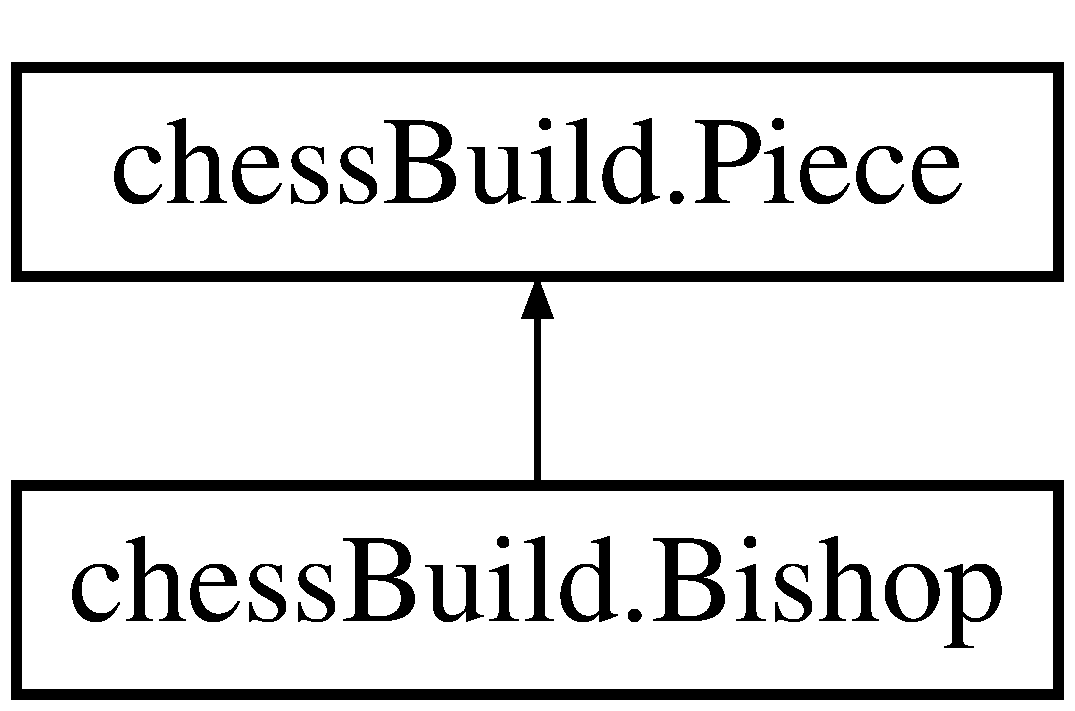
\includegraphics[height=2.000000cm]{classchess_build_1_1_bishop}
\end{center}
\end{figure}
\subsection*{Public Member Functions}
\begin{DoxyCompactItemize}
\item 
\hyperlink{classchess_build_1_1_bishop_abcd27a8cfe14ac745b82b1235975dfe5}{Bishop} ()
\item 
\hyperlink{classchess_build_1_1_bishop_abd25029ee4ece2514a31704c77136eab}{Bishop} (\hyperlink{classchess_build_1_1_bishop}{Bishop} other)
\item 
\hyperlink{classchess_build_1_1_bishop_a89d83da5ab8ceb0fc56b16684009631e}{Bishop} (String color)
\item 
\hyperlink{classchess_build_1_1_bishop_a33e408253263931181c912a9addf6e2b}{Bishop} (int x, int y, String color, boolean is\+Alive)
\item 
\mbox{\Hypertarget{classchess_build_1_1_bishop_a349fcd0bc55597d24908a45bd200e685}\label{classchess_build_1_1_bishop_a349fcd0bc55597d24908a45bd200e685}} 
boolean {\bfseries check\+Move} (\hyperlink{classchess_build_1_1_board}{Board} board, int targetX, int targetY)
\item 
boolean \hyperlink{classchess_build_1_1_bishop_a59cd9646587b373feff0cd2e743fa434}{check\+Bishop\+Move\+Helper} (\hyperlink{classchess_build_1_1_board}{Board} board, int targetX, int targetY)
\end{DoxyCompactItemize}


\subsection{Constructor \& Destructor Documentation}
\mbox{\Hypertarget{classchess_build_1_1_bishop_abcd27a8cfe14ac745b82b1235975dfe5}\label{classchess_build_1_1_bishop_abcd27a8cfe14ac745b82b1235975dfe5}} 
\index{chess\+Build\+::\+Bishop@{chess\+Build\+::\+Bishop}!Bishop@{Bishop}}
\index{Bishop@{Bishop}!chess\+Build\+::\+Bishop@{chess\+Build\+::\+Bishop}}
\subsubsection{\texorpdfstring{Bishop()}{Bishop()}\hspace{0.1cm}{\footnotesize\ttfamily [1/4]}}
{\footnotesize\ttfamily chess\+Build.\+Bishop.\+Bishop (\begin{DoxyParamCaption}{ }\end{DoxyParamCaption})}

Default Constructor \mbox{\Hypertarget{classchess_build_1_1_bishop_abd25029ee4ece2514a31704c77136eab}\label{classchess_build_1_1_bishop_abd25029ee4ece2514a31704c77136eab}} 
\index{chess\+Build\+::\+Bishop@{chess\+Build\+::\+Bishop}!Bishop@{Bishop}}
\index{Bishop@{Bishop}!chess\+Build\+::\+Bishop@{chess\+Build\+::\+Bishop}}
\subsubsection{\texorpdfstring{Bishop()}{Bishop()}\hspace{0.1cm}{\footnotesize\ttfamily [2/4]}}
{\footnotesize\ttfamily chess\+Build.\+Bishop.\+Bishop (\begin{DoxyParamCaption}\item[{\hyperlink{classchess_build_1_1_bishop}{Bishop}}]{other }\end{DoxyParamCaption})}

Copy constructor 
\begin{DoxyParams}{Parameters}
{\em other} & \\
\hline
\end{DoxyParams}
\mbox{\Hypertarget{classchess_build_1_1_bishop_a89d83da5ab8ceb0fc56b16684009631e}\label{classchess_build_1_1_bishop_a89d83da5ab8ceb0fc56b16684009631e}} 
\index{chess\+Build\+::\+Bishop@{chess\+Build\+::\+Bishop}!Bishop@{Bishop}}
\index{Bishop@{Bishop}!chess\+Build\+::\+Bishop@{chess\+Build\+::\+Bishop}}
\subsubsection{\texorpdfstring{Bishop()}{Bishop()}\hspace{0.1cm}{\footnotesize\ttfamily [3/4]}}
{\footnotesize\ttfamily chess\+Build.\+Bishop.\+Bishop (\begin{DoxyParamCaption}\item[{String}]{color }\end{DoxyParamCaption})}

\hyperlink{classchess_build_1_1_bishop}{Bishop} constructor 
\begin{DoxyParams}{Parameters}
{\em color} & \\
\hline
\end{DoxyParams}
\mbox{\Hypertarget{classchess_build_1_1_bishop_a33e408253263931181c912a9addf6e2b}\label{classchess_build_1_1_bishop_a33e408253263931181c912a9addf6e2b}} 
\index{chess\+Build\+::\+Bishop@{chess\+Build\+::\+Bishop}!Bishop@{Bishop}}
\index{Bishop@{Bishop}!chess\+Build\+::\+Bishop@{chess\+Build\+::\+Bishop}}
\subsubsection{\texorpdfstring{Bishop()}{Bishop()}\hspace{0.1cm}{\footnotesize\ttfamily [4/4]}}
{\footnotesize\ttfamily chess\+Build.\+Bishop.\+Bishop (\begin{DoxyParamCaption}\item[{int}]{x,  }\item[{int}]{y,  }\item[{String}]{color,  }\item[{boolean}]{is\+Alive }\end{DoxyParamCaption})}

\hyperlink{classchess_build_1_1_bishop}{Bishop} constructor 
\begin{DoxyParams}{Parameters}
{\em x} & \\
\hline
{\em y} & \\
\hline
{\em color} & \\
\hline
{\em is\+Alive} & \\
\hline
\end{DoxyParams}


\subsection{Member Function Documentation}
\mbox{\Hypertarget{classchess_build_1_1_bishop_a59cd9646587b373feff0cd2e743fa434}\label{classchess_build_1_1_bishop_a59cd9646587b373feff0cd2e743fa434}} 
\index{chess\+Build\+::\+Bishop@{chess\+Build\+::\+Bishop}!check\+Bishop\+Move\+Helper@{check\+Bishop\+Move\+Helper}}
\index{check\+Bishop\+Move\+Helper@{check\+Bishop\+Move\+Helper}!chess\+Build\+::\+Bishop@{chess\+Build\+::\+Bishop}}
\subsubsection{\texorpdfstring{check\+Bishop\+Move\+Helper()}{checkBishopMoveHelper()}}
{\footnotesize\ttfamily boolean chess\+Build.\+Bishop.\+check\+Bishop\+Move\+Helper (\begin{DoxyParamCaption}\item[{\hyperlink{classchess_build_1_1_board}{Board}}]{board,  }\item[{int}]{targetX,  }\item[{int}]{targetY }\end{DoxyParamCaption})}

Helper method for check\+Move function for \hyperlink{classchess_build_1_1_bishop}{Bishop} 
\begin{DoxyParams}{Parameters}
{\em board} & \\
\hline
{\em targetX} & \\
\hline
{\em targetY} & \\
\hline
\end{DoxyParams}
\begin{DoxyReturn}{Returns}

\end{DoxyReturn}


The documentation for this class was generated from the following file\+:\begin{DoxyCompactItemize}
\item 
src/chess\+Build/Bishop.\+java\end{DoxyCompactItemize}

\hypertarget{classchess_build_1_1_board}{}\section{chess\+Build.\+Board Class Reference}
\label{classchess_build_1_1_board}\index{chess\+Build.\+Board@{chess\+Build.\+Board}}
\subsection*{Public Member Functions}
\begin{DoxyCompactItemize}
\item 
\hyperlink{classchess_build_1_1_board_a41548dc02b3082c7a8f93a02919ec564}{Board} (int row, int column)
\item 
\hyperlink{classchess_build_1_1_board_a07018ac4fd8680cf86449f9446f81e9d}{Board} (\hyperlink{classchess_build_1_1_board}{Board} other)
\item 
\hyperlink{classchess_build_1_1_piece}{Piece} \hyperlink{classchess_build_1_1_board_ad0b01d5dfb0e517bc41593f57d2cc073}{get\+Piece} (int x, int y)
\item 
void \hyperlink{classchess_build_1_1_board_a1b83ee1026b863cb830768d555906931}{set\+Row} (int row)
\item 
int \hyperlink{classchess_build_1_1_board_a7d54f83b6a633d9d6eb39220a99e67ef}{get\+Row} ()
\item 
void \hyperlink{classchess_build_1_1_board_a946a842a42f1f5f172901232e13a4eff}{set\+Column} (int column)
\item 
int \hyperlink{classchess_build_1_1_board_a90f2eeba043a2a1524e350a745610da7}{get\+Column} ()
\item 
void \hyperlink{classchess_build_1_1_board_ad3229351025edaff14e166ab1c7bd5b9}{set\+Chess\+Board} (\hyperlink{classchess_build_1_1_piece}{Piece} p, int x, int y)
\item 
\hyperlink{classchess_build_1_1_piece}{Piece} \hyperlink{classchess_build_1_1_board_ac58d9824c7dc8ee3449896ae38802f22}{get\+Chess\+Board} (int x, int y)
\end{DoxyCompactItemize}
\subsection*{Public Attributes}
\begin{DoxyCompactItemize}
\item 
\mbox{\Hypertarget{classchess_build_1_1_board_ae059d3225c704edb16a4cd5c38bb3698}\label{classchess_build_1_1_board_ae059d3225c704edb16a4cd5c38bb3698}} 
\hyperlink{classchess_build_1_1_piece}{Piece} {\bfseries chess\+Board} \mbox{[}$\,$\mbox{]}\mbox{[}$\,$\mbox{]}
\end{DoxyCompactItemize}


\subsection{Constructor \& Destructor Documentation}
\mbox{\Hypertarget{classchess_build_1_1_board_a41548dc02b3082c7a8f93a02919ec564}\label{classchess_build_1_1_board_a41548dc02b3082c7a8f93a02919ec564}} 
\index{chess\+Build\+::\+Board@{chess\+Build\+::\+Board}!Board@{Board}}
\index{Board@{Board}!chess\+Build\+::\+Board@{chess\+Build\+::\+Board}}
\subsubsection{\texorpdfstring{Board()}{Board()}\hspace{0.1cm}{\footnotesize\ttfamily [1/2]}}
{\footnotesize\ttfamily chess\+Build.\+Board.\+Board (\begin{DoxyParamCaption}\item[{int}]{row,  }\item[{int}]{column }\end{DoxyParamCaption})}

Constructor for board 
\begin{DoxyParams}{Parameters}
{\em row} & \\
\hline
{\em column} & \\
\hline
\end{DoxyParams}
\mbox{\Hypertarget{classchess_build_1_1_board_a07018ac4fd8680cf86449f9446f81e9d}\label{classchess_build_1_1_board_a07018ac4fd8680cf86449f9446f81e9d}} 
\index{chess\+Build\+::\+Board@{chess\+Build\+::\+Board}!Board@{Board}}
\index{Board@{Board}!chess\+Build\+::\+Board@{chess\+Build\+::\+Board}}
\subsubsection{\texorpdfstring{Board()}{Board()}\hspace{0.1cm}{\footnotesize\ttfamily [2/2]}}
{\footnotesize\ttfamily chess\+Build.\+Board.\+Board (\begin{DoxyParamCaption}\item[{\hyperlink{classchess_build_1_1_board}{Board}}]{other }\end{DoxyParamCaption})}

Copy constructor 
\begin{DoxyParams}{Parameters}
{\em other} & \\
\hline
\end{DoxyParams}


\subsection{Member Function Documentation}
\mbox{\Hypertarget{classchess_build_1_1_board_ac58d9824c7dc8ee3449896ae38802f22}\label{classchess_build_1_1_board_ac58d9824c7dc8ee3449896ae38802f22}} 
\index{chess\+Build\+::\+Board@{chess\+Build\+::\+Board}!get\+Chess\+Board@{get\+Chess\+Board}}
\index{get\+Chess\+Board@{get\+Chess\+Board}!chess\+Build\+::\+Board@{chess\+Build\+::\+Board}}
\subsubsection{\texorpdfstring{get\+Chess\+Board()}{getChessBoard()}}
{\footnotesize\ttfamily \hyperlink{classchess_build_1_1_piece}{Piece} chess\+Build.\+Board.\+get\+Chess\+Board (\begin{DoxyParamCaption}\item[{int}]{x,  }\item[{int}]{y }\end{DoxyParamCaption})}

Get the piece of board 
\begin{DoxyParams}{Parameters}
{\em x} & \\
\hline
{\em y} & \\
\hline
\end{DoxyParams}
\begin{DoxyReturn}{Returns}

\end{DoxyReturn}
\mbox{\Hypertarget{classchess_build_1_1_board_a90f2eeba043a2a1524e350a745610da7}\label{classchess_build_1_1_board_a90f2eeba043a2a1524e350a745610da7}} 
\index{chess\+Build\+::\+Board@{chess\+Build\+::\+Board}!get\+Column@{get\+Column}}
\index{get\+Column@{get\+Column}!chess\+Build\+::\+Board@{chess\+Build\+::\+Board}}
\subsubsection{\texorpdfstring{get\+Column()}{getColumn()}}
{\footnotesize\ttfamily int chess\+Build.\+Board.\+get\+Column (\begin{DoxyParamCaption}{ }\end{DoxyParamCaption})}

Get the column of board \begin{DoxyReturn}{Returns}

\end{DoxyReturn}
\mbox{\Hypertarget{classchess_build_1_1_board_ad0b01d5dfb0e517bc41593f57d2cc073}\label{classchess_build_1_1_board_ad0b01d5dfb0e517bc41593f57d2cc073}} 
\index{chess\+Build\+::\+Board@{chess\+Build\+::\+Board}!get\+Piece@{get\+Piece}}
\index{get\+Piece@{get\+Piece}!chess\+Build\+::\+Board@{chess\+Build\+::\+Board}}
\subsubsection{\texorpdfstring{get\+Piece()}{getPiece()}}
{\footnotesize\ttfamily \hyperlink{classchess_build_1_1_piece}{Piece} chess\+Build.\+Board.\+get\+Piece (\begin{DoxyParamCaption}\item[{int}]{x,  }\item[{int}]{y }\end{DoxyParamCaption})}

Get the piece on the board 
\begin{DoxyParams}{Parameters}
{\em x} & \\
\hline
{\em y} & \\
\hline
\end{DoxyParams}
\begin{DoxyReturn}{Returns}

\end{DoxyReturn}
\mbox{\Hypertarget{classchess_build_1_1_board_a7d54f83b6a633d9d6eb39220a99e67ef}\label{classchess_build_1_1_board_a7d54f83b6a633d9d6eb39220a99e67ef}} 
\index{chess\+Build\+::\+Board@{chess\+Build\+::\+Board}!get\+Row@{get\+Row}}
\index{get\+Row@{get\+Row}!chess\+Build\+::\+Board@{chess\+Build\+::\+Board}}
\subsubsection{\texorpdfstring{get\+Row()}{getRow()}}
{\footnotesize\ttfamily int chess\+Build.\+Board.\+get\+Row (\begin{DoxyParamCaption}{ }\end{DoxyParamCaption})}

Get the row of board \begin{DoxyReturn}{Returns}

\end{DoxyReturn}
\mbox{\Hypertarget{classchess_build_1_1_board_ad3229351025edaff14e166ab1c7bd5b9}\label{classchess_build_1_1_board_ad3229351025edaff14e166ab1c7bd5b9}} 
\index{chess\+Build\+::\+Board@{chess\+Build\+::\+Board}!set\+Chess\+Board@{set\+Chess\+Board}}
\index{set\+Chess\+Board@{set\+Chess\+Board}!chess\+Build\+::\+Board@{chess\+Build\+::\+Board}}
\subsubsection{\texorpdfstring{set\+Chess\+Board()}{setChessBoard()}}
{\footnotesize\ttfamily void chess\+Build.\+Board.\+set\+Chess\+Board (\begin{DoxyParamCaption}\item[{\hyperlink{classchess_build_1_1_piece}{Piece}}]{p,  }\item[{int}]{x,  }\item[{int}]{y }\end{DoxyParamCaption})}

Set the piece of board 
\begin{DoxyParams}{Parameters}
{\em p} & \\
\hline
{\em x} & \\
\hline
{\em y} & \\
\hline
\end{DoxyParams}
\mbox{\Hypertarget{classchess_build_1_1_board_a946a842a42f1f5f172901232e13a4eff}\label{classchess_build_1_1_board_a946a842a42f1f5f172901232e13a4eff}} 
\index{chess\+Build\+::\+Board@{chess\+Build\+::\+Board}!set\+Column@{set\+Column}}
\index{set\+Column@{set\+Column}!chess\+Build\+::\+Board@{chess\+Build\+::\+Board}}
\subsubsection{\texorpdfstring{set\+Column()}{setColumn()}}
{\footnotesize\ttfamily void chess\+Build.\+Board.\+set\+Column (\begin{DoxyParamCaption}\item[{int}]{column }\end{DoxyParamCaption})}

Set the column of board 
\begin{DoxyParams}{Parameters}
{\em column} & \\
\hline
\end{DoxyParams}
\mbox{\Hypertarget{classchess_build_1_1_board_a1b83ee1026b863cb830768d555906931}\label{classchess_build_1_1_board_a1b83ee1026b863cb830768d555906931}} 
\index{chess\+Build\+::\+Board@{chess\+Build\+::\+Board}!set\+Row@{set\+Row}}
\index{set\+Row@{set\+Row}!chess\+Build\+::\+Board@{chess\+Build\+::\+Board}}
\subsubsection{\texorpdfstring{set\+Row()}{setRow()}}
{\footnotesize\ttfamily void chess\+Build.\+Board.\+set\+Row (\begin{DoxyParamCaption}\item[{int}]{row }\end{DoxyParamCaption})}

Set the row of board 
\begin{DoxyParams}{Parameters}
{\em row} & \\
\hline
\end{DoxyParams}


The documentation for this class was generated from the following file\+:\begin{DoxyCompactItemize}
\item 
src/chess\+Build/Board.\+java\end{DoxyCompactItemize}

\hypertarget{classchess_g_u_i_1_1_control}{}\section{chess\+G\+U\+I.\+Control Class Reference}
\label{classchess_g_u_i_1_1_control}\index{chess\+G\+U\+I.\+Control@{chess\+G\+U\+I.\+Control}}
Inheritance diagram for chess\+G\+U\+I.\+Control\+:\begin{figure}[H]
\begin{center}
\leavevmode
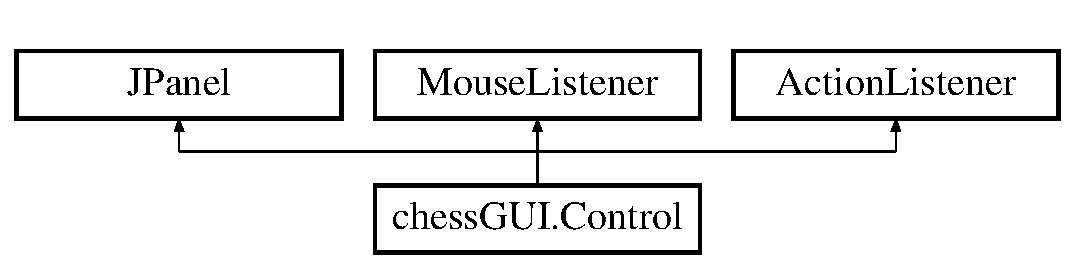
\includegraphics[height=2.000000cm]{classchess_g_u_i_1_1_control}
\end{center}
\end{figure}
\subsection*{Public Member Functions}
\begin{DoxyCompactItemize}
\item 
\hyperlink{classchess_g_u_i_1_1_control_ac90efc0d259e84d21ffa95fac1e63d42}{Control} ()
\item 
void \hyperlink{classchess_g_u_i_1_1_control_aa88e3fa81b7dbfc40cd2b1bfaf120ab0}{paint} (Graphics g)
\item 
\mbox{\Hypertarget{classchess_g_u_i_1_1_control_a4bab2ca00238562006756235c286b75e}\label{classchess_g_u_i_1_1_control_a4bab2ca00238562006756235c286b75e}} 
void {\bfseries mouse\+Clicked} (Mouse\+Event e)
\item 
\mbox{\Hypertarget{classchess_g_u_i_1_1_control_a6b61da8fee1e978ce060e05b27c5d046}\label{classchess_g_u_i_1_1_control_a6b61da8fee1e978ce060e05b27c5d046}} 
void {\bfseries mouse\+Pressed} (Mouse\+Event e)
\item 
\mbox{\Hypertarget{classchess_g_u_i_1_1_control_a78abefe1216996058ae02642007eb08e}\label{classchess_g_u_i_1_1_control_a78abefe1216996058ae02642007eb08e}} 
void {\bfseries mouse\+Released} (Mouse\+Event e)
\item 
\mbox{\Hypertarget{classchess_g_u_i_1_1_control_a7840821c207d7c130ffea346361ffcea}\label{classchess_g_u_i_1_1_control_a7840821c207d7c130ffea346361ffcea}} 
void {\bfseries mouse\+Entered} (Mouse\+Event e)
\item 
\mbox{\Hypertarget{classchess_g_u_i_1_1_control_a7fe35c1e0306eca7455730b169a2e70f}\label{classchess_g_u_i_1_1_control_a7fe35c1e0306eca7455730b169a2e70f}} 
void {\bfseries mouse\+Exited} (Mouse\+Event e)
\item 
\mbox{\Hypertarget{classchess_g_u_i_1_1_control_afca86d2c9603a9d15539a3fcad1b7708}\label{classchess_g_u_i_1_1_control_afca86d2c9603a9d15539a3fcad1b7708}} 
void {\bfseries action\+Performed} (Action\+Event e)
\end{DoxyCompactItemize}
\subsection*{Static Public Attributes}
\begin{DoxyCompactItemize}
\item 
\mbox{\Hypertarget{classchess_g_u_i_1_1_control_a3cfa23bfb0c24f9f4518336ff7bc0317}\label{classchess_g_u_i_1_1_control_a3cfa23bfb0c24f9f4518336ff7bc0317}} 
static boolean {\bfseries start\+Game} = false
\item 
\mbox{\Hypertarget{classchess_g_u_i_1_1_control_a8e1a9728ff532915917a1ba7d56647f3}\label{classchess_g_u_i_1_1_control_a8e1a9728ff532915917a1ba7d56647f3}} 
static \hyperlink{classchess_build_1_1_game}{Game} {\bfseries game} = new \hyperlink{classchess_build_1_1_game}{Game}()
\item 
\mbox{\Hypertarget{classchess_g_u_i_1_1_control_aeeb4b2ebf477ff865e7ec04878f0203d}\label{classchess_g_u_i_1_1_control_aeeb4b2ebf477ff865e7ec04878f0203d}} 
static Stack$<$ \hyperlink{classchess_build_1_1_game}{Game} $>$ {\bfseries last\+Move} = new Stack$<$\hyperlink{classchess_build_1_1_game}{Game}$>$()
\end{DoxyCompactItemize}


\subsection{Constructor \& Destructor Documentation}
\mbox{\Hypertarget{classchess_g_u_i_1_1_control_ac90efc0d259e84d21ffa95fac1e63d42}\label{classchess_g_u_i_1_1_control_ac90efc0d259e84d21ffa95fac1e63d42}} 
\index{chess\+G\+U\+I\+::\+Control@{chess\+G\+U\+I\+::\+Control}!Control@{Control}}
\index{Control@{Control}!chess\+G\+U\+I\+::\+Control@{chess\+G\+U\+I\+::\+Control}}
\subsubsection{\texorpdfstring{Control()}{Control()}}
{\footnotesize\ttfamily chess\+G\+U\+I.\+Control.\+Control (\begin{DoxyParamCaption}{ }\end{DoxyParamCaption})}

\hyperlink{classchess_g_u_i_1_1_control}{Control} constructor 

\subsection{Member Function Documentation}
\mbox{\Hypertarget{classchess_g_u_i_1_1_control_aa88e3fa81b7dbfc40cd2b1bfaf120ab0}\label{classchess_g_u_i_1_1_control_aa88e3fa81b7dbfc40cd2b1bfaf120ab0}} 
\index{chess\+G\+U\+I\+::\+Control@{chess\+G\+U\+I\+::\+Control}!paint@{paint}}
\index{paint@{paint}!chess\+G\+U\+I\+::\+Control@{chess\+G\+U\+I\+::\+Control}}
\subsubsection{\texorpdfstring{paint()}{paint()}}
{\footnotesize\ttfamily void chess\+G\+U\+I.\+Control.\+paint (\begin{DoxyParamCaption}\item[{Graphics}]{g }\end{DoxyParamCaption})}

New Piece// 

The documentation for this class was generated from the following file\+:\begin{DoxyCompactItemize}
\item 
src/chess\+G\+U\+I/Control.\+java\end{DoxyCompactItemize}

\hypertarget{classchess_build_1_1_elephant}{}\section{chess\+Build.\+Elephant Class Reference}
\label{classchess_build_1_1_elephant}\index{chess\+Build.\+Elephant@{chess\+Build.\+Elephant}}
Inheritance diagram for chess\+Build.\+Elephant\+:\begin{figure}[H]
\begin{center}
\leavevmode
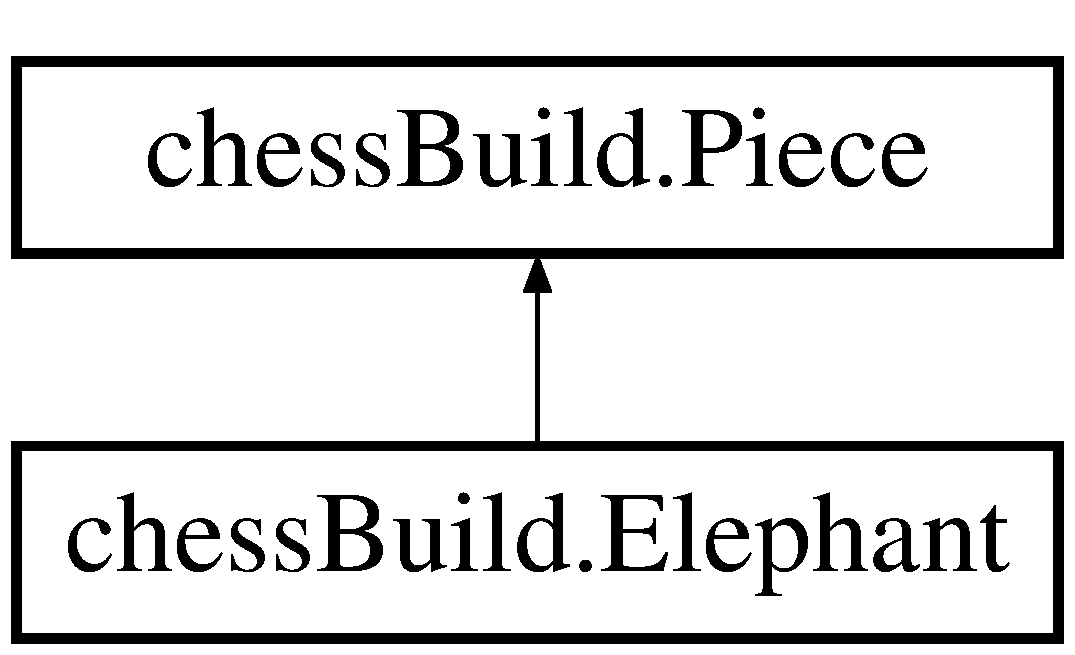
\includegraphics[height=2.000000cm]{classchess_build_1_1_elephant}
\end{center}
\end{figure}
\subsection*{Public Member Functions}
\begin{DoxyCompactItemize}
\item 
\hyperlink{classchess_build_1_1_elephant_a10ef050e05cb57bace154ff12752115b}{Elephant} ()
\item 
\hyperlink{classchess_build_1_1_elephant_ac60142f5a3931dbbf71ecc65358d43a3}{Elephant} (String color)
\item 
\hyperlink{classchess_build_1_1_elephant_a0323849e4a8078589161ab4d684f56ce}{Elephant} (\hyperlink{classchess_build_1_1_elephant}{Elephant} other)
\item 
\hyperlink{classchess_build_1_1_elephant_ad32f3bcb8f925d0d0a0e26285b2009f3}{Elephant} (int x, int y, String color, boolean is\+Alive)
\item 
\mbox{\Hypertarget{classchess_build_1_1_elephant_a576a8241d17268a8d070b41d96f15832}\label{classchess_build_1_1_elephant_a576a8241d17268a8d070b41d96f15832}} 
boolean {\bfseries check\+Move} (\hyperlink{classchess_build_1_1_board}{Board} board, int targetX, int targetY)
\item 
boolean \hyperlink{classchess_build_1_1_elephant_a2385d9354fdc457beee06e59f2da8464}{check\+Elephant\+Move\+Helper} (\hyperlink{classchess_build_1_1_board}{Board} board, int targetX, int targetY)
\end{DoxyCompactItemize}


\subsection{Constructor \& Destructor Documentation}
\mbox{\Hypertarget{classchess_build_1_1_elephant_a10ef050e05cb57bace154ff12752115b}\label{classchess_build_1_1_elephant_a10ef050e05cb57bace154ff12752115b}} 
\index{chess\+Build\+::\+Elephant@{chess\+Build\+::\+Elephant}!Elephant@{Elephant}}
\index{Elephant@{Elephant}!chess\+Build\+::\+Elephant@{chess\+Build\+::\+Elephant}}
\subsubsection{\texorpdfstring{Elephant()}{Elephant()}\hspace{0.1cm}{\footnotesize\ttfamily [1/4]}}
{\footnotesize\ttfamily chess\+Build.\+Elephant.\+Elephant (\begin{DoxyParamCaption}{ }\end{DoxyParamCaption})}

Default constructor \mbox{\Hypertarget{classchess_build_1_1_elephant_ac60142f5a3931dbbf71ecc65358d43a3}\label{classchess_build_1_1_elephant_ac60142f5a3931dbbf71ecc65358d43a3}} 
\index{chess\+Build\+::\+Elephant@{chess\+Build\+::\+Elephant}!Elephant@{Elephant}}
\index{Elephant@{Elephant}!chess\+Build\+::\+Elephant@{chess\+Build\+::\+Elephant}}
\subsubsection{\texorpdfstring{Elephant()}{Elephant()}\hspace{0.1cm}{\footnotesize\ttfamily [2/4]}}
{\footnotesize\ttfamily chess\+Build.\+Elephant.\+Elephant (\begin{DoxyParamCaption}\item[{String}]{color }\end{DoxyParamCaption})}

\hyperlink{classchess_build_1_1_elephant}{Elephant} constructor 
\begin{DoxyParams}{Parameters}
{\em color} & \\
\hline
\end{DoxyParams}
\mbox{\Hypertarget{classchess_build_1_1_elephant_a0323849e4a8078589161ab4d684f56ce}\label{classchess_build_1_1_elephant_a0323849e4a8078589161ab4d684f56ce}} 
\index{chess\+Build\+::\+Elephant@{chess\+Build\+::\+Elephant}!Elephant@{Elephant}}
\index{Elephant@{Elephant}!chess\+Build\+::\+Elephant@{chess\+Build\+::\+Elephant}}
\subsubsection{\texorpdfstring{Elephant()}{Elephant()}\hspace{0.1cm}{\footnotesize\ttfamily [3/4]}}
{\footnotesize\ttfamily chess\+Build.\+Elephant.\+Elephant (\begin{DoxyParamCaption}\item[{\hyperlink{classchess_build_1_1_elephant}{Elephant}}]{other }\end{DoxyParamCaption})}

Copy constructor 
\begin{DoxyParams}{Parameters}
{\em other} & \\
\hline
\end{DoxyParams}
\mbox{\Hypertarget{classchess_build_1_1_elephant_ad32f3bcb8f925d0d0a0e26285b2009f3}\label{classchess_build_1_1_elephant_ad32f3bcb8f925d0d0a0e26285b2009f3}} 
\index{chess\+Build\+::\+Elephant@{chess\+Build\+::\+Elephant}!Elephant@{Elephant}}
\index{Elephant@{Elephant}!chess\+Build\+::\+Elephant@{chess\+Build\+::\+Elephant}}
\subsubsection{\texorpdfstring{Elephant()}{Elephant()}\hspace{0.1cm}{\footnotesize\ttfamily [4/4]}}
{\footnotesize\ttfamily chess\+Build.\+Elephant.\+Elephant (\begin{DoxyParamCaption}\item[{int}]{x,  }\item[{int}]{y,  }\item[{String}]{color,  }\item[{boolean}]{is\+Alive }\end{DoxyParamCaption})}

\hyperlink{classchess_build_1_1_elephant}{Elephant} constructor 
\begin{DoxyParams}{Parameters}
{\em x} & \\
\hline
{\em y} & \\
\hline
{\em color} & \\
\hline
{\em is\+Alive} & \\
\hline
\end{DoxyParams}


\subsection{Member Function Documentation}
\mbox{\Hypertarget{classchess_build_1_1_elephant_a2385d9354fdc457beee06e59f2da8464}\label{classchess_build_1_1_elephant_a2385d9354fdc457beee06e59f2da8464}} 
\index{chess\+Build\+::\+Elephant@{chess\+Build\+::\+Elephant}!check\+Elephant\+Move\+Helper@{check\+Elephant\+Move\+Helper}}
\index{check\+Elephant\+Move\+Helper@{check\+Elephant\+Move\+Helper}!chess\+Build\+::\+Elephant@{chess\+Build\+::\+Elephant}}
\subsubsection{\texorpdfstring{check\+Elephant\+Move\+Helper()}{checkElephantMoveHelper()}}
{\footnotesize\ttfamily boolean chess\+Build.\+Elephant.\+check\+Elephant\+Move\+Helper (\begin{DoxyParamCaption}\item[{\hyperlink{classchess_build_1_1_board}{Board}}]{board,  }\item[{int}]{targetX,  }\item[{int}]{targetY }\end{DoxyParamCaption})}

Helper function for check\+Move method 
\begin{DoxyParams}{Parameters}
{\em board} & \\
\hline
{\em targetX} & \\
\hline
{\em targetY} & \\
\hline
\end{DoxyParams}
\begin{DoxyReturn}{Returns}

\end{DoxyReturn}


The documentation for this class was generated from the following file\+:\begin{DoxyCompactItemize}
\item 
src/chess\+Build/Elephant.\+java\end{DoxyCompactItemize}

\hypertarget{classchess_build_1_1_game}{}\section{chess\+Build.\+Game Class Reference}
\label{classchess_build_1_1_game}\index{chess\+Build.\+Game@{chess\+Build.\+Game}}
\subsection*{Public Member Functions}
\begin{DoxyCompactItemize}
\item 
\hyperlink{classchess_build_1_1_game_aaaf23256b0a8d37893c6671d17e7a163}{Game} ()
\item 
\hyperlink{classchess_build_1_1_game_a0d9475651b9d1824074a45bae670c03a}{Game} (\hyperlink{classchess_build_1_1_game}{Game} other)
\item 
void \hyperlink{classchess_build_1_1_game_a5a575d1b5298b7ddee17f08a1784153b}{initialize\+Game} ()
\item 
String \hyperlink{classchess_build_1_1_game_af10e6d9b2b1192e1381a4ae3cffbca5c}{get\+Winner} ()
\item 
void \hyperlink{classchess_build_1_1_game_a6bc01e50f0e37b437db78cb029807d25}{set\+Winner} (String win)
\item 
\hyperlink{classchess_build_1_1_player}{Player} \hyperlink{classchess_build_1_1_game_aa2ae560bff80ac9628ffee5b4fa57b33}{get\+White\+Player} ()
\item 
\hyperlink{classchess_build_1_1_player}{Player} \hyperlink{classchess_build_1_1_game_a1aa884addf9d116b66cd8643995144a4}{get\+Black\+Player} ()
\item 
int \hyperlink{classchess_build_1_1_game_a6271b0abcddb945758b3a70ec3a2be47}{get\+Row} ()
\item 
int \hyperlink{classchess_build_1_1_game_a6c917e051708604f5385062146e2880c}{get\+Column} ()
\item 
boolean \hyperlink{classchess_build_1_1_game_abf2a3e04a58e0ed986dc5951002b3af6}{get\+Game\+End} ()
\item 
void \hyperlink{classchess_build_1_1_game_ac6400be2899f19c3ee57cc5946ea4154}{set\+Game\+End} (boolean end)
\item 
boolean \hyperlink{classchess_build_1_1_game_a5ef5fc90fd60545c3b70a1eff98ce306}{get\+White\+Turn} ()
\item 
void \hyperlink{classchess_build_1_1_game_a32d1a61488dc1af6c1d33c3ff2f40bd1}{set\+White\+Turn} (boolean turn)
\item 
void \hyperlink{classchess_build_1_1_game_ae396b8c108a1fc863db4ae1a665de341}{initialize\+Chess\+Board} ()
\item 
void \hyperlink{classchess_build_1_1_game_a11ff0646f34a1aec27b9153c135ed0ba}{initialize\+Black\+Player} ()
\item 
void \hyperlink{classchess_build_1_1_game_ae164441ea754520c20538fcb304ff2d5}{initialize\+White\+Player} ()
\item 
void \hyperlink{classchess_build_1_1_game_ace070bfd577b47865b05b2220048bb0c}{move\+Piece} (int currX, int currY, int targetX, int targetY)
\item 
boolean \hyperlink{classchess_build_1_1_game_a58ffbacab5b8755dd53248b635329807}{move\+Piece\+Helper} (int currX, int currY, int targetX, int targetY)
\item 
void \hyperlink{classchess_build_1_1_game_a7191ea6816333cc8b6d6994e8241f0b5}{white\+Move} (int currX, int currY, int targetX, int targetY)
\item 
void \hyperlink{classchess_build_1_1_game_a42ebac6f010a92be253e201f06fd0487}{black\+Move} (int currX, int currY, int targetX, int targetY)
\item 
boolean \hyperlink{classchess_build_1_1_game_aeb3f335df2f0143f39c6654d02b77a97}{check\+Mate} (\hyperlink{classchess_build_1_1_player}{Player} player)
\item 
boolean \hyperlink{classchess_build_1_1_game_a2e93dda47c0e5c8ec8c7cc234c048b9e}{safe\+Position} (\hyperlink{classchess_build_1_1_player}{Player} player, int x, int y)
\item 
boolean \hyperlink{classchess_build_1_1_game_a594c69523dbb0732107f9809d9c6a80e}{check\+King\+Target\+Position} (\hyperlink{classchess_build_1_1_player}{Player} player, int currX, int currY, int targetX, int targetY)
\item 
void \hyperlink{classchess_build_1_1_game_a873c004e82d9a3bed1f8dec57b781ee5}{change\+Version} ()
\end{DoxyCompactItemize}
\subsection*{Public Attributes}
\begin{DoxyCompactItemize}
\item 
\mbox{\Hypertarget{classchess_build_1_1_game_a4b725ab015366deb0a7253ad676cc063}\label{classchess_build_1_1_game_a4b725ab015366deb0a7253ad676cc063}} 
\hyperlink{classchess_build_1_1_board}{Board} {\bfseries board}
\end{DoxyCompactItemize}


\subsection{Constructor \& Destructor Documentation}
\mbox{\Hypertarget{classchess_build_1_1_game_aaaf23256b0a8d37893c6671d17e7a163}\label{classchess_build_1_1_game_aaaf23256b0a8d37893c6671d17e7a163}} 
\index{chess\+Build\+::\+Game@{chess\+Build\+::\+Game}!Game@{Game}}
\index{Game@{Game}!chess\+Build\+::\+Game@{chess\+Build\+::\+Game}}
\subsubsection{\texorpdfstring{Game()}{Game()}\hspace{0.1cm}{\footnotesize\ttfamily [1/2]}}
{\footnotesize\ttfamily chess\+Build.\+Game.\+Game (\begin{DoxyParamCaption}{ }\end{DoxyParamCaption})}

Default constructor of game \mbox{\Hypertarget{classchess_build_1_1_game_a0d9475651b9d1824074a45bae670c03a}\label{classchess_build_1_1_game_a0d9475651b9d1824074a45bae670c03a}} 
\index{chess\+Build\+::\+Game@{chess\+Build\+::\+Game}!Game@{Game}}
\index{Game@{Game}!chess\+Build\+::\+Game@{chess\+Build\+::\+Game}}
\subsubsection{\texorpdfstring{Game()}{Game()}\hspace{0.1cm}{\footnotesize\ttfamily [2/2]}}
{\footnotesize\ttfamily chess\+Build.\+Game.\+Game (\begin{DoxyParamCaption}\item[{\hyperlink{classchess_build_1_1_game}{Game}}]{other }\end{DoxyParamCaption})}

Copy constructor 
\begin{DoxyParams}{Parameters}
{\em other} & \\
\hline
\end{DoxyParams}


\subsection{Member Function Documentation}
\mbox{\Hypertarget{classchess_build_1_1_game_a42ebac6f010a92be253e201f06fd0487}\label{classchess_build_1_1_game_a42ebac6f010a92be253e201f06fd0487}} 
\index{chess\+Build\+::\+Game@{chess\+Build\+::\+Game}!black\+Move@{black\+Move}}
\index{black\+Move@{black\+Move}!chess\+Build\+::\+Game@{chess\+Build\+::\+Game}}
\subsubsection{\texorpdfstring{black\+Move()}{blackMove()}}
{\footnotesize\ttfamily void chess\+Build.\+Game.\+black\+Move (\begin{DoxyParamCaption}\item[{int}]{currX,  }\item[{int}]{currY,  }\item[{int}]{targetX,  }\item[{int}]{targetY }\end{DoxyParamCaption})}

Move the black piece 
\begin{DoxyParams}{Parameters}
{\em currX} & \\
\hline
{\em currY} & \\
\hline
{\em targetX} & \\
\hline
{\em targetY} & \\
\hline
\end{DoxyParams}
\mbox{\Hypertarget{classchess_build_1_1_game_a873c004e82d9a3bed1f8dec57b781ee5}\label{classchess_build_1_1_game_a873c004e82d9a3bed1f8dec57b781ee5}} 
\index{chess\+Build\+::\+Game@{chess\+Build\+::\+Game}!change\+Version@{change\+Version}}
\index{change\+Version@{change\+Version}!chess\+Build\+::\+Game@{chess\+Build\+::\+Game}}
\subsubsection{\texorpdfstring{change\+Version()}{changeVersion()}}
{\footnotesize\ttfamily void chess\+Build.\+Game.\+change\+Version (\begin{DoxyParamCaption}{ }\end{DoxyParamCaption})}

This method changes the version of the game by replacing original piece knight with new piece kin and elephant. \mbox{\Hypertarget{classchess_build_1_1_game_a594c69523dbb0732107f9809d9c6a80e}\label{classchess_build_1_1_game_a594c69523dbb0732107f9809d9c6a80e}} 
\index{chess\+Build\+::\+Game@{chess\+Build\+::\+Game}!check\+King\+Target\+Position@{check\+King\+Target\+Position}}
\index{check\+King\+Target\+Position@{check\+King\+Target\+Position}!chess\+Build\+::\+Game@{chess\+Build\+::\+Game}}
\subsubsection{\texorpdfstring{check\+King\+Target\+Position()}{checkKingTargetPosition()}}
{\footnotesize\ttfamily boolean chess\+Build.\+Game.\+check\+King\+Target\+Position (\begin{DoxyParamCaption}\item[{\hyperlink{classchess_build_1_1_player}{Player}}]{player,  }\item[{int}]{currX,  }\item[{int}]{currY,  }\item[{int}]{targetX,  }\item[{int}]{targetY }\end{DoxyParamCaption})}

Check whether the target place of king is dangerous 
\begin{DoxyParams}{Parameters}
{\em player} & \\
\hline
{\em currX} & \\
\hline
{\em currY} & \\
\hline
{\em targetX} & \\
\hline
{\em targetY} & \\
\hline
\end{DoxyParams}
\begin{DoxyReturn}{Returns}

\end{DoxyReturn}
\mbox{\Hypertarget{classchess_build_1_1_game_aeb3f335df2f0143f39c6654d02b77a97}\label{classchess_build_1_1_game_aeb3f335df2f0143f39c6654d02b77a97}} 
\index{chess\+Build\+::\+Game@{chess\+Build\+::\+Game}!check\+Mate@{check\+Mate}}
\index{check\+Mate@{check\+Mate}!chess\+Build\+::\+Game@{chess\+Build\+::\+Game}}
\subsubsection{\texorpdfstring{check\+Mate()}{checkMate()}}
{\footnotesize\ttfamily boolean chess\+Build.\+Game.\+check\+Mate (\begin{DoxyParamCaption}\item[{\hyperlink{classchess_build_1_1_player}{Player}}]{player }\end{DoxyParamCaption})}

Check\+Mate function for the game 
\begin{DoxyParams}{Parameters}
{\em player} & \\
\hline
\end{DoxyParams}
\begin{DoxyReturn}{Returns}

\end{DoxyReturn}
\mbox{\Hypertarget{classchess_build_1_1_game_a1aa884addf9d116b66cd8643995144a4}\label{classchess_build_1_1_game_a1aa884addf9d116b66cd8643995144a4}} 
\index{chess\+Build\+::\+Game@{chess\+Build\+::\+Game}!get\+Black\+Player@{get\+Black\+Player}}
\index{get\+Black\+Player@{get\+Black\+Player}!chess\+Build\+::\+Game@{chess\+Build\+::\+Game}}
\subsubsection{\texorpdfstring{get\+Black\+Player()}{getBlackPlayer()}}
{\footnotesize\ttfamily \hyperlink{classchess_build_1_1_player}{Player} chess\+Build.\+Game.\+get\+Black\+Player (\begin{DoxyParamCaption}{ }\end{DoxyParamCaption})}

Get the black player of the game \begin{DoxyReturn}{Returns}

\end{DoxyReturn}
\mbox{\Hypertarget{classchess_build_1_1_game_a6c917e051708604f5385062146e2880c}\label{classchess_build_1_1_game_a6c917e051708604f5385062146e2880c}} 
\index{chess\+Build\+::\+Game@{chess\+Build\+::\+Game}!get\+Column@{get\+Column}}
\index{get\+Column@{get\+Column}!chess\+Build\+::\+Game@{chess\+Build\+::\+Game}}
\subsubsection{\texorpdfstring{get\+Column()}{getColumn()}}
{\footnotesize\ttfamily int chess\+Build.\+Game.\+get\+Column (\begin{DoxyParamCaption}{ }\end{DoxyParamCaption})}

Get the column \begin{DoxyReturn}{Returns}

\end{DoxyReturn}
\mbox{\Hypertarget{classchess_build_1_1_game_abf2a3e04a58e0ed986dc5951002b3af6}\label{classchess_build_1_1_game_abf2a3e04a58e0ed986dc5951002b3af6}} 
\index{chess\+Build\+::\+Game@{chess\+Build\+::\+Game}!get\+Game\+End@{get\+Game\+End}}
\index{get\+Game\+End@{get\+Game\+End}!chess\+Build\+::\+Game@{chess\+Build\+::\+Game}}
\subsubsection{\texorpdfstring{get\+Game\+End()}{getGameEnd()}}
{\footnotesize\ttfamily boolean chess\+Build.\+Game.\+get\+Game\+End (\begin{DoxyParamCaption}{ }\end{DoxyParamCaption})}

Get the game\+End \begin{DoxyReturn}{Returns}

\end{DoxyReturn}
\mbox{\Hypertarget{classchess_build_1_1_game_a6271b0abcddb945758b3a70ec3a2be47}\label{classchess_build_1_1_game_a6271b0abcddb945758b3a70ec3a2be47}} 
\index{chess\+Build\+::\+Game@{chess\+Build\+::\+Game}!get\+Row@{get\+Row}}
\index{get\+Row@{get\+Row}!chess\+Build\+::\+Game@{chess\+Build\+::\+Game}}
\subsubsection{\texorpdfstring{get\+Row()}{getRow()}}
{\footnotesize\ttfamily int chess\+Build.\+Game.\+get\+Row (\begin{DoxyParamCaption}{ }\end{DoxyParamCaption})}

Get the row \begin{DoxyReturn}{Returns}

\end{DoxyReturn}
\mbox{\Hypertarget{classchess_build_1_1_game_aa2ae560bff80ac9628ffee5b4fa57b33}\label{classchess_build_1_1_game_aa2ae560bff80ac9628ffee5b4fa57b33}} 
\index{chess\+Build\+::\+Game@{chess\+Build\+::\+Game}!get\+White\+Player@{get\+White\+Player}}
\index{get\+White\+Player@{get\+White\+Player}!chess\+Build\+::\+Game@{chess\+Build\+::\+Game}}
\subsubsection{\texorpdfstring{get\+White\+Player()}{getWhitePlayer()}}
{\footnotesize\ttfamily \hyperlink{classchess_build_1_1_player}{Player} chess\+Build.\+Game.\+get\+White\+Player (\begin{DoxyParamCaption}{ }\end{DoxyParamCaption})}

Get the white player of the game \begin{DoxyReturn}{Returns}

\end{DoxyReturn}
\mbox{\Hypertarget{classchess_build_1_1_game_a5ef5fc90fd60545c3b70a1eff98ce306}\label{classchess_build_1_1_game_a5ef5fc90fd60545c3b70a1eff98ce306}} 
\index{chess\+Build\+::\+Game@{chess\+Build\+::\+Game}!get\+White\+Turn@{get\+White\+Turn}}
\index{get\+White\+Turn@{get\+White\+Turn}!chess\+Build\+::\+Game@{chess\+Build\+::\+Game}}
\subsubsection{\texorpdfstring{get\+White\+Turn()}{getWhiteTurn()}}
{\footnotesize\ttfamily boolean chess\+Build.\+Game.\+get\+White\+Turn (\begin{DoxyParamCaption}{ }\end{DoxyParamCaption})}

Get the turn of player \begin{DoxyReturn}{Returns}

\end{DoxyReturn}
\mbox{\Hypertarget{classchess_build_1_1_game_af10e6d9b2b1192e1381a4ae3cffbca5c}\label{classchess_build_1_1_game_af10e6d9b2b1192e1381a4ae3cffbca5c}} 
\index{chess\+Build\+::\+Game@{chess\+Build\+::\+Game}!get\+Winner@{get\+Winner}}
\index{get\+Winner@{get\+Winner}!chess\+Build\+::\+Game@{chess\+Build\+::\+Game}}
\subsubsection{\texorpdfstring{get\+Winner()}{getWinner()}}
{\footnotesize\ttfamily String chess\+Build.\+Game.\+get\+Winner (\begin{DoxyParamCaption}{ }\end{DoxyParamCaption})}

Get winner method \begin{DoxyReturn}{Returns}

\end{DoxyReturn}
\mbox{\Hypertarget{classchess_build_1_1_game_a11ff0646f34a1aec27b9153c135ed0ba}\label{classchess_build_1_1_game_a11ff0646f34a1aec27b9153c135ed0ba}} 
\index{chess\+Build\+::\+Game@{chess\+Build\+::\+Game}!initialize\+Black\+Player@{initialize\+Black\+Player}}
\index{initialize\+Black\+Player@{initialize\+Black\+Player}!chess\+Build\+::\+Game@{chess\+Build\+::\+Game}}
\subsubsection{\texorpdfstring{initialize\+Black\+Player()}{initializeBlackPlayer()}}
{\footnotesize\ttfamily void chess\+Build.\+Game.\+initialize\+Black\+Player (\begin{DoxyParamCaption}{ }\end{DoxyParamCaption})}

Initialize the black\+Player of the game \mbox{\Hypertarget{classchess_build_1_1_game_ae396b8c108a1fc863db4ae1a665de341}\label{classchess_build_1_1_game_ae396b8c108a1fc863db4ae1a665de341}} 
\index{chess\+Build\+::\+Game@{chess\+Build\+::\+Game}!initialize\+Chess\+Board@{initialize\+Chess\+Board}}
\index{initialize\+Chess\+Board@{initialize\+Chess\+Board}!chess\+Build\+::\+Game@{chess\+Build\+::\+Game}}
\subsubsection{\texorpdfstring{initialize\+Chess\+Board()}{initializeChessBoard()}}
{\footnotesize\ttfamily void chess\+Build.\+Game.\+initialize\+Chess\+Board (\begin{DoxyParamCaption}{ }\end{DoxyParamCaption})}

Initialize the board of the game \mbox{\Hypertarget{classchess_build_1_1_game_a5a575d1b5298b7ddee17f08a1784153b}\label{classchess_build_1_1_game_a5a575d1b5298b7ddee17f08a1784153b}} 
\index{chess\+Build\+::\+Game@{chess\+Build\+::\+Game}!initialize\+Game@{initialize\+Game}}
\index{initialize\+Game@{initialize\+Game}!chess\+Build\+::\+Game@{chess\+Build\+::\+Game}}
\subsubsection{\texorpdfstring{initialize\+Game()}{initializeGame()}}
{\footnotesize\ttfamily void chess\+Build.\+Game.\+initialize\+Game (\begin{DoxyParamCaption}{ }\end{DoxyParamCaption})}

Initialize the game \mbox{\Hypertarget{classchess_build_1_1_game_ae164441ea754520c20538fcb304ff2d5}\label{classchess_build_1_1_game_ae164441ea754520c20538fcb304ff2d5}} 
\index{chess\+Build\+::\+Game@{chess\+Build\+::\+Game}!initialize\+White\+Player@{initialize\+White\+Player}}
\index{initialize\+White\+Player@{initialize\+White\+Player}!chess\+Build\+::\+Game@{chess\+Build\+::\+Game}}
\subsubsection{\texorpdfstring{initialize\+White\+Player()}{initializeWhitePlayer()}}
{\footnotesize\ttfamily void chess\+Build.\+Game.\+initialize\+White\+Player (\begin{DoxyParamCaption}{ }\end{DoxyParamCaption})}

Initialize the white player of the game \mbox{\Hypertarget{classchess_build_1_1_game_ace070bfd577b47865b05b2220048bb0c}\label{classchess_build_1_1_game_ace070bfd577b47865b05b2220048bb0c}} 
\index{chess\+Build\+::\+Game@{chess\+Build\+::\+Game}!move\+Piece@{move\+Piece}}
\index{move\+Piece@{move\+Piece}!chess\+Build\+::\+Game@{chess\+Build\+::\+Game}}
\subsubsection{\texorpdfstring{move\+Piece()}{movePiece()}}
{\footnotesize\ttfamily void chess\+Build.\+Game.\+move\+Piece (\begin{DoxyParamCaption}\item[{int}]{currX,  }\item[{int}]{currY,  }\item[{int}]{targetX,  }\item[{int}]{targetY }\end{DoxyParamCaption})}

This function move the piece on the board by taking the initial position and target position 
\begin{DoxyParams}{Parameters}
{\em currX} & \\
\hline
{\em currY} & \\
\hline
{\em targetX} & \\
\hline
{\em targetY} & \\
\hline
\end{DoxyParams}
\mbox{\Hypertarget{classchess_build_1_1_game_a58ffbacab5b8755dd53248b635329807}\label{classchess_build_1_1_game_a58ffbacab5b8755dd53248b635329807}} 
\index{chess\+Build\+::\+Game@{chess\+Build\+::\+Game}!move\+Piece\+Helper@{move\+Piece\+Helper}}
\index{move\+Piece\+Helper@{move\+Piece\+Helper}!chess\+Build\+::\+Game@{chess\+Build\+::\+Game}}
\subsubsection{\texorpdfstring{move\+Piece\+Helper()}{movePieceHelper()}}
{\footnotesize\ttfamily boolean chess\+Build.\+Game.\+move\+Piece\+Helper (\begin{DoxyParamCaption}\item[{int}]{currX,  }\item[{int}]{currY,  }\item[{int}]{targetX,  }\item[{int}]{targetY }\end{DoxyParamCaption})}

The function will return false if the input is invalid 
\begin{DoxyParams}{Parameters}
{\em currX} & \\
\hline
{\em currY} & \\
\hline
{\em targetX} & \\
\hline
{\em targetY} & \\
\hline
\end{DoxyParams}
\begin{DoxyReturn}{Returns}

\end{DoxyReturn}
\mbox{\Hypertarget{classchess_build_1_1_game_a2e93dda47c0e5c8ec8c7cc234c048b9e}\label{classchess_build_1_1_game_a2e93dda47c0e5c8ec8c7cc234c048b9e}} 
\index{chess\+Build\+::\+Game@{chess\+Build\+::\+Game}!safe\+Position@{safe\+Position}}
\index{safe\+Position@{safe\+Position}!chess\+Build\+::\+Game@{chess\+Build\+::\+Game}}
\subsubsection{\texorpdfstring{safe\+Position()}{safePosition()}}
{\footnotesize\ttfamily boolean chess\+Build.\+Game.\+safe\+Position (\begin{DoxyParamCaption}\item[{\hyperlink{classchess_build_1_1_player}{Player}}]{player,  }\item[{int}]{x,  }\item[{int}]{y }\end{DoxyParamCaption})}

The function checks whether the selected position is safe for the player 
\begin{DoxyParams}{Parameters}
{\em player} & \\
\hline
{\em x} & \\
\hline
{\em y} & \\
\hline
\end{DoxyParams}
\begin{DoxyReturn}{Returns}

\end{DoxyReturn}
\mbox{\Hypertarget{classchess_build_1_1_game_ac6400be2899f19c3ee57cc5946ea4154}\label{classchess_build_1_1_game_ac6400be2899f19c3ee57cc5946ea4154}} 
\index{chess\+Build\+::\+Game@{chess\+Build\+::\+Game}!set\+Game\+End@{set\+Game\+End}}
\index{set\+Game\+End@{set\+Game\+End}!chess\+Build\+::\+Game@{chess\+Build\+::\+Game}}
\subsubsection{\texorpdfstring{set\+Game\+End()}{setGameEnd()}}
{\footnotesize\ttfamily void chess\+Build.\+Game.\+set\+Game\+End (\begin{DoxyParamCaption}\item[{boolean}]{end }\end{DoxyParamCaption})}

Set the game\+End 
\begin{DoxyParams}{Parameters}
{\em end} & \\
\hline
\end{DoxyParams}
\mbox{\Hypertarget{classchess_build_1_1_game_a32d1a61488dc1af6c1d33c3ff2f40bd1}\label{classchess_build_1_1_game_a32d1a61488dc1af6c1d33c3ff2f40bd1}} 
\index{chess\+Build\+::\+Game@{chess\+Build\+::\+Game}!set\+White\+Turn@{set\+White\+Turn}}
\index{set\+White\+Turn@{set\+White\+Turn}!chess\+Build\+::\+Game@{chess\+Build\+::\+Game}}
\subsubsection{\texorpdfstring{set\+White\+Turn()}{setWhiteTurn()}}
{\footnotesize\ttfamily void chess\+Build.\+Game.\+set\+White\+Turn (\begin{DoxyParamCaption}\item[{boolean}]{turn }\end{DoxyParamCaption})}

Set the turn of player 
\begin{DoxyParams}{Parameters}
{\em turn} & \\
\hline
\end{DoxyParams}
\mbox{\Hypertarget{classchess_build_1_1_game_a6bc01e50f0e37b437db78cb029807d25}\label{classchess_build_1_1_game_a6bc01e50f0e37b437db78cb029807d25}} 
\index{chess\+Build\+::\+Game@{chess\+Build\+::\+Game}!set\+Winner@{set\+Winner}}
\index{set\+Winner@{set\+Winner}!chess\+Build\+::\+Game@{chess\+Build\+::\+Game}}
\subsubsection{\texorpdfstring{set\+Winner()}{setWinner()}}
{\footnotesize\ttfamily void chess\+Build.\+Game.\+set\+Winner (\begin{DoxyParamCaption}\item[{String}]{win }\end{DoxyParamCaption})}

Set the winner of the game 
\begin{DoxyParams}{Parameters}
{\em win} & \\
\hline
\end{DoxyParams}
\mbox{\Hypertarget{classchess_build_1_1_game_a7191ea6816333cc8b6d6994e8241f0b5}\label{classchess_build_1_1_game_a7191ea6816333cc8b6d6994e8241f0b5}} 
\index{chess\+Build\+::\+Game@{chess\+Build\+::\+Game}!white\+Move@{white\+Move}}
\index{white\+Move@{white\+Move}!chess\+Build\+::\+Game@{chess\+Build\+::\+Game}}
\subsubsection{\texorpdfstring{white\+Move()}{whiteMove()}}
{\footnotesize\ttfamily void chess\+Build.\+Game.\+white\+Move (\begin{DoxyParamCaption}\item[{int}]{currX,  }\item[{int}]{currY,  }\item[{int}]{targetX,  }\item[{int}]{targetY }\end{DoxyParamCaption})}

Move the white \hyperlink{classchess_build_1_1_piece}{Piece} 
\begin{DoxyParams}{Parameters}
{\em currX} & \\
\hline
{\em currY} & \\
\hline
{\em targetX} & \\
\hline
{\em targetY} & \\
\hline
\end{DoxyParams}


The documentation for this class was generated from the following file\+:\begin{DoxyCompactItemize}
\item 
src/chess\+Build/Game.\+java\end{DoxyCompactItemize}

\hypertarget{classchess_build_1_1_kin}{}\section{chess\+Build.\+Kin Class Reference}
\label{classchess_build_1_1_kin}\index{chess\+Build.\+Kin@{chess\+Build.\+Kin}}
Inheritance diagram for chess\+Build.\+Kin\+:\begin{figure}[H]
\begin{center}
\leavevmode
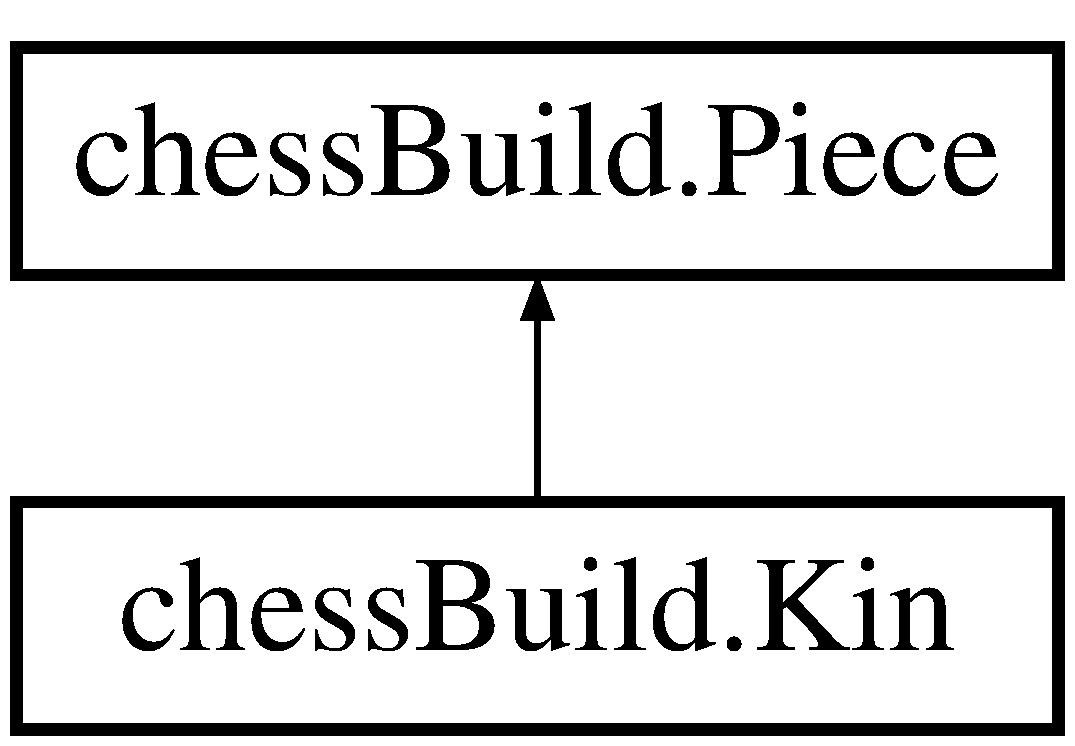
\includegraphics[height=2.000000cm]{classchess_build_1_1_kin}
\end{center}
\end{figure}
\subsection*{Public Member Functions}
\begin{DoxyCompactItemize}
\item 
\hyperlink{classchess_build_1_1_kin_a87a23160a9f1f1de6671115fcc381d2a}{Kin} ()
\item 
\hyperlink{classchess_build_1_1_kin_a62136f6aa7070fecc551dedb629a4838}{Kin} (\hyperlink{classchess_build_1_1_kin}{Kin} other)
\item 
\hyperlink{classchess_build_1_1_kin_acd1bc04a123663cf9c7bb8c0e20ede24}{Kin} (String color)
\item 
\hyperlink{classchess_build_1_1_kin_a1618ef88cbfbbb03ecbb6f03965d802a}{Kin} (int x, int y, String color, boolean is\+Alive)
\item 
\mbox{\Hypertarget{classchess_build_1_1_kin_a7e6a78d6c00f2065c5b65d41220a943a}\label{classchess_build_1_1_kin_a7e6a78d6c00f2065c5b65d41220a943a}} 
boolean {\bfseries check\+Move} (\hyperlink{classchess_build_1_1_board}{Board} board, int targetX, int targetY)
\item 
boolean \hyperlink{classchess_build_1_1_kin_ae8873f13b3785528b9bc34ac2b9efa9a}{check\+Kin\+Move\+Helper} (\hyperlink{classchess_build_1_1_board}{Board} board, int targetX, int targetY)
\end{DoxyCompactItemize}


\subsection{Constructor \& Destructor Documentation}
\mbox{\Hypertarget{classchess_build_1_1_kin_a87a23160a9f1f1de6671115fcc381d2a}\label{classchess_build_1_1_kin_a87a23160a9f1f1de6671115fcc381d2a}} 
\index{chess\+Build\+::\+Kin@{chess\+Build\+::\+Kin}!Kin@{Kin}}
\index{Kin@{Kin}!chess\+Build\+::\+Kin@{chess\+Build\+::\+Kin}}
\subsubsection{\texorpdfstring{Kin()}{Kin()}\hspace{0.1cm}{\footnotesize\ttfamily [1/4]}}
{\footnotesize\ttfamily chess\+Build.\+Kin.\+Kin (\begin{DoxyParamCaption}{ }\end{DoxyParamCaption})}

Default constructor \mbox{\Hypertarget{classchess_build_1_1_kin_a62136f6aa7070fecc551dedb629a4838}\label{classchess_build_1_1_kin_a62136f6aa7070fecc551dedb629a4838}} 
\index{chess\+Build\+::\+Kin@{chess\+Build\+::\+Kin}!Kin@{Kin}}
\index{Kin@{Kin}!chess\+Build\+::\+Kin@{chess\+Build\+::\+Kin}}
\subsubsection{\texorpdfstring{Kin()}{Kin()}\hspace{0.1cm}{\footnotesize\ttfamily [2/4]}}
{\footnotesize\ttfamily chess\+Build.\+Kin.\+Kin (\begin{DoxyParamCaption}\item[{\hyperlink{classchess_build_1_1_kin}{Kin}}]{other }\end{DoxyParamCaption})}

Copy constructor 
\begin{DoxyParams}{Parameters}
{\em other} & \\
\hline
\end{DoxyParams}
\mbox{\Hypertarget{classchess_build_1_1_kin_acd1bc04a123663cf9c7bb8c0e20ede24}\label{classchess_build_1_1_kin_acd1bc04a123663cf9c7bb8c0e20ede24}} 
\index{chess\+Build\+::\+Kin@{chess\+Build\+::\+Kin}!Kin@{Kin}}
\index{Kin@{Kin}!chess\+Build\+::\+Kin@{chess\+Build\+::\+Kin}}
\subsubsection{\texorpdfstring{Kin()}{Kin()}\hspace{0.1cm}{\footnotesize\ttfamily [3/4]}}
{\footnotesize\ttfamily chess\+Build.\+Kin.\+Kin (\begin{DoxyParamCaption}\item[{String}]{color }\end{DoxyParamCaption})}

\hyperlink{classchess_build_1_1_kin}{Kin} constructor 
\begin{DoxyParams}{Parameters}
{\em color} & \\
\hline
\end{DoxyParams}
\mbox{\Hypertarget{classchess_build_1_1_kin_a1618ef88cbfbbb03ecbb6f03965d802a}\label{classchess_build_1_1_kin_a1618ef88cbfbbb03ecbb6f03965d802a}} 
\index{chess\+Build\+::\+Kin@{chess\+Build\+::\+Kin}!Kin@{Kin}}
\index{Kin@{Kin}!chess\+Build\+::\+Kin@{chess\+Build\+::\+Kin}}
\subsubsection{\texorpdfstring{Kin()}{Kin()}\hspace{0.1cm}{\footnotesize\ttfamily [4/4]}}
{\footnotesize\ttfamily chess\+Build.\+Kin.\+Kin (\begin{DoxyParamCaption}\item[{int}]{x,  }\item[{int}]{y,  }\item[{String}]{color,  }\item[{boolean}]{is\+Alive }\end{DoxyParamCaption})}

\hyperlink{classchess_build_1_1_kin}{Kin} constructor 
\begin{DoxyParams}{Parameters}
{\em x} & \\
\hline
{\em y} & \\
\hline
{\em color} & \\
\hline
{\em is\+Alive} & \\
\hline
\end{DoxyParams}


\subsection{Member Function Documentation}
\mbox{\Hypertarget{classchess_build_1_1_kin_ae8873f13b3785528b9bc34ac2b9efa9a}\label{classchess_build_1_1_kin_ae8873f13b3785528b9bc34ac2b9efa9a}} 
\index{chess\+Build\+::\+Kin@{chess\+Build\+::\+Kin}!check\+Kin\+Move\+Helper@{check\+Kin\+Move\+Helper}}
\index{check\+Kin\+Move\+Helper@{check\+Kin\+Move\+Helper}!chess\+Build\+::\+Kin@{chess\+Build\+::\+Kin}}
\subsubsection{\texorpdfstring{check\+Kin\+Move\+Helper()}{checkKinMoveHelper()}}
{\footnotesize\ttfamily boolean chess\+Build.\+Kin.\+check\+Kin\+Move\+Helper (\begin{DoxyParamCaption}\item[{\hyperlink{classchess_build_1_1_board}{Board}}]{board,  }\item[{int}]{targetX,  }\item[{int}]{targetY }\end{DoxyParamCaption})}

Helper function for check\+Move method 
\begin{DoxyParams}{Parameters}
{\em board} & \\
\hline
{\em targetX} & \\
\hline
{\em targetY} & \\
\hline
\end{DoxyParams}
\begin{DoxyReturn}{Returns}

\end{DoxyReturn}


The documentation for this class was generated from the following file\+:\begin{DoxyCompactItemize}
\item 
src/chess\+Build/Kin.\+java\end{DoxyCompactItemize}

\hypertarget{classchess_build_1_1_king}{}\section{chess\+Build.\+King Class Reference}
\label{classchess_build_1_1_king}\index{chess\+Build.\+King@{chess\+Build.\+King}}
Inheritance diagram for chess\+Build.\+King\+:\begin{figure}[H]
\begin{center}
\leavevmode
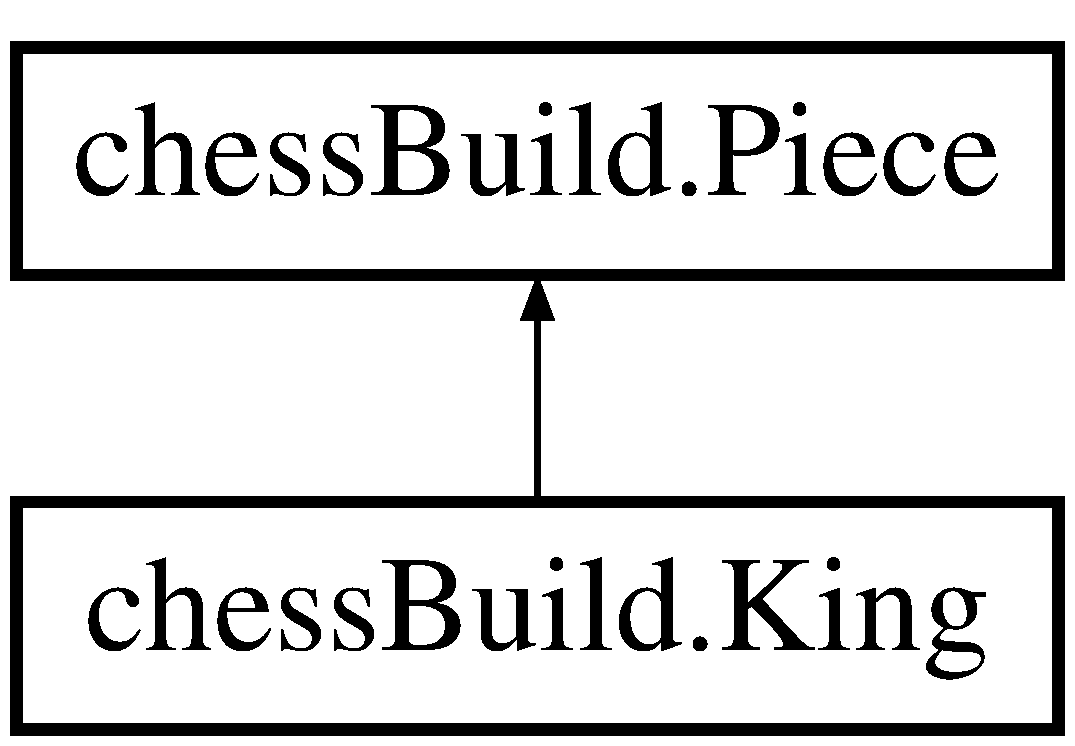
\includegraphics[height=2.000000cm]{classchess_build_1_1_king}
\end{center}
\end{figure}
\subsection*{Public Member Functions}
\begin{DoxyCompactItemize}
\item 
\hyperlink{classchess_build_1_1_king_a9d47020d3baaa12653e51f3eec27e9b1}{King} ()
\item 
\hyperlink{classchess_build_1_1_king_ad07e90a3afe7fed1830d734dbd4817a8}{King} (\hyperlink{classchess_build_1_1_king}{King} other)
\item 
\hyperlink{classchess_build_1_1_king_a24d4ed37d11c00c7475ed7fe529ece66}{King} (String color)
\item 
\hyperlink{classchess_build_1_1_king_a3f2ec37749356fa6f5faaabaa0bb2d07}{King} (int x, int y, String color, boolean is\+Alive)
\item 
\mbox{\Hypertarget{classchess_build_1_1_king_a41d9aba602d97e747e20fae592a4378c}\label{classchess_build_1_1_king_a41d9aba602d97e747e20fae592a4378c}} 
boolean {\bfseries check\+Move} (\hyperlink{classchess_build_1_1_board}{Board} board, int targetX, int targetY)
\item 
boolean \hyperlink{classchess_build_1_1_king_aceffd2bb1fe5398fac99961e70420e39}{check\+King\+Move\+Helper} (\hyperlink{classchess_build_1_1_board}{Board} board, int targetX, int targetY)
\end{DoxyCompactItemize}


\subsection{Constructor \& Destructor Documentation}
\mbox{\Hypertarget{classchess_build_1_1_king_a9d47020d3baaa12653e51f3eec27e9b1}\label{classchess_build_1_1_king_a9d47020d3baaa12653e51f3eec27e9b1}} 
\index{chess\+Build\+::\+King@{chess\+Build\+::\+King}!King@{King}}
\index{King@{King}!chess\+Build\+::\+King@{chess\+Build\+::\+King}}
\subsubsection{\texorpdfstring{King()}{King()}\hspace{0.1cm}{\footnotesize\ttfamily [1/4]}}
{\footnotesize\ttfamily chess\+Build.\+King.\+King (\begin{DoxyParamCaption}{ }\end{DoxyParamCaption})}

Default Constructor \mbox{\Hypertarget{classchess_build_1_1_king_ad07e90a3afe7fed1830d734dbd4817a8}\label{classchess_build_1_1_king_ad07e90a3afe7fed1830d734dbd4817a8}} 
\index{chess\+Build\+::\+King@{chess\+Build\+::\+King}!King@{King}}
\index{King@{King}!chess\+Build\+::\+King@{chess\+Build\+::\+King}}
\subsubsection{\texorpdfstring{King()}{King()}\hspace{0.1cm}{\footnotesize\ttfamily [2/4]}}
{\footnotesize\ttfamily chess\+Build.\+King.\+King (\begin{DoxyParamCaption}\item[{\hyperlink{classchess_build_1_1_king}{King}}]{other }\end{DoxyParamCaption})}

Copy constructor 
\begin{DoxyParams}{Parameters}
{\em other} & \\
\hline
\end{DoxyParams}
\mbox{\Hypertarget{classchess_build_1_1_king_a24d4ed37d11c00c7475ed7fe529ece66}\label{classchess_build_1_1_king_a24d4ed37d11c00c7475ed7fe529ece66}} 
\index{chess\+Build\+::\+King@{chess\+Build\+::\+King}!King@{King}}
\index{King@{King}!chess\+Build\+::\+King@{chess\+Build\+::\+King}}
\subsubsection{\texorpdfstring{King()}{King()}\hspace{0.1cm}{\footnotesize\ttfamily [3/4]}}
{\footnotesize\ttfamily chess\+Build.\+King.\+King (\begin{DoxyParamCaption}\item[{String}]{color }\end{DoxyParamCaption})}

Constructor for king 
\begin{DoxyParams}{Parameters}
{\em color} & \\
\hline
\end{DoxyParams}
\mbox{\Hypertarget{classchess_build_1_1_king_a3f2ec37749356fa6f5faaabaa0bb2d07}\label{classchess_build_1_1_king_a3f2ec37749356fa6f5faaabaa0bb2d07}} 
\index{chess\+Build\+::\+King@{chess\+Build\+::\+King}!King@{King}}
\index{King@{King}!chess\+Build\+::\+King@{chess\+Build\+::\+King}}
\subsubsection{\texorpdfstring{King()}{King()}\hspace{0.1cm}{\footnotesize\ttfamily [4/4]}}
{\footnotesize\ttfamily chess\+Build.\+King.\+King (\begin{DoxyParamCaption}\item[{int}]{x,  }\item[{int}]{y,  }\item[{String}]{color,  }\item[{boolean}]{is\+Alive }\end{DoxyParamCaption})}

Constructor for \hyperlink{classchess_build_1_1_king}{King} 
\begin{DoxyParams}{Parameters}
{\em x} & \\
\hline
{\em y} & \\
\hline
{\em color} & \\
\hline
{\em is\+Alive} & \\
\hline
\end{DoxyParams}


\subsection{Member Function Documentation}
\mbox{\Hypertarget{classchess_build_1_1_king_aceffd2bb1fe5398fac99961e70420e39}\label{classchess_build_1_1_king_aceffd2bb1fe5398fac99961e70420e39}} 
\index{chess\+Build\+::\+King@{chess\+Build\+::\+King}!check\+King\+Move\+Helper@{check\+King\+Move\+Helper}}
\index{check\+King\+Move\+Helper@{check\+King\+Move\+Helper}!chess\+Build\+::\+King@{chess\+Build\+::\+King}}
\subsubsection{\texorpdfstring{check\+King\+Move\+Helper()}{checkKingMoveHelper()}}
{\footnotesize\ttfamily boolean chess\+Build.\+King.\+check\+King\+Move\+Helper (\begin{DoxyParamCaption}\item[{\hyperlink{classchess_build_1_1_board}{Board}}]{board,  }\item[{int}]{targetX,  }\item[{int}]{targetY }\end{DoxyParamCaption})}

Helper function for check\+Move method 
\begin{DoxyParams}{Parameters}
{\em board} & \\
\hline
{\em targetX} & \\
\hline
{\em targetY} & \\
\hline
\end{DoxyParams}
\begin{DoxyReturn}{Returns}

\end{DoxyReturn}


The documentation for this class was generated from the following file\+:\begin{DoxyCompactItemize}
\item 
src/chess\+Build/King.\+java\end{DoxyCompactItemize}

\hypertarget{classchess_build_1_1_knight}{}\section{chess\+Build.\+Knight Class Reference}
\label{classchess_build_1_1_knight}\index{chess\+Build.\+Knight@{chess\+Build.\+Knight}}
Inheritance diagram for chess\+Build.\+Knight\+:\begin{figure}[H]
\begin{center}
\leavevmode
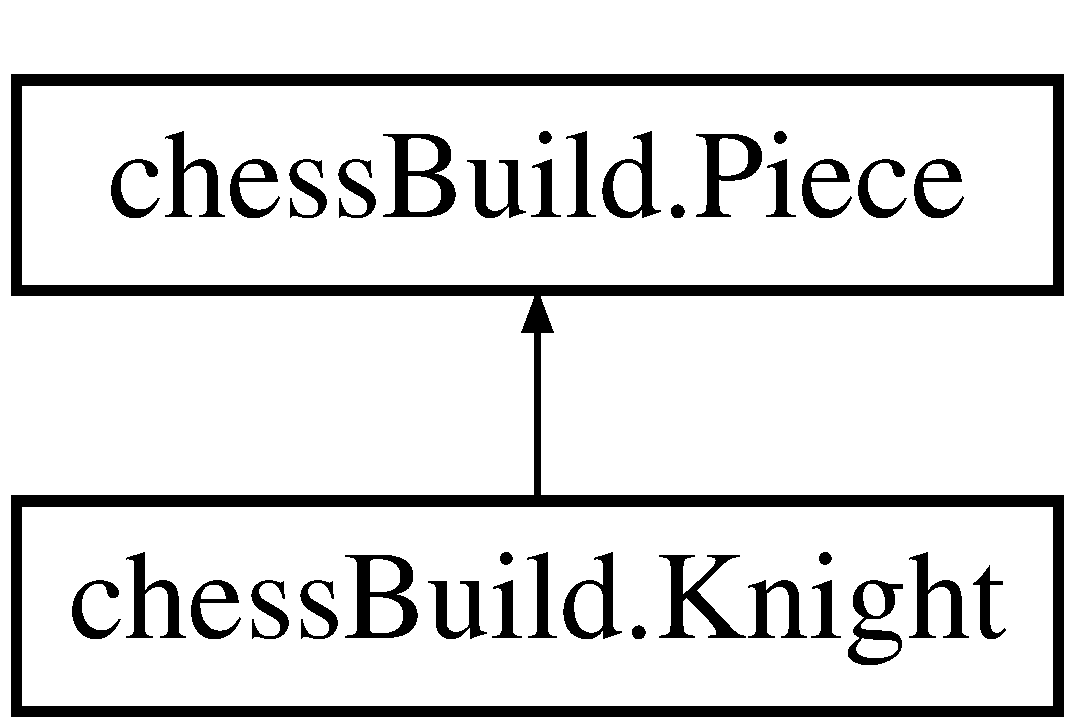
\includegraphics[height=2.000000cm]{classchess_build_1_1_knight}
\end{center}
\end{figure}
\subsection*{Public Member Functions}
\begin{DoxyCompactItemize}
\item 
\hyperlink{classchess_build_1_1_knight_ae863e0fcef4d27a72dbbc1d70eed38a0}{Knight} ()
\item 
\hyperlink{classchess_build_1_1_knight_ad282a386bcf3eb2550bb0ddbaedb4fef}{Knight} (\hyperlink{classchess_build_1_1_knight}{Knight} other)
\item 
\hyperlink{classchess_build_1_1_knight_a52b03f556c615328116b62f3f2c4bb0a}{Knight} (String color)
\item 
\hyperlink{classchess_build_1_1_knight_af9b14f7aa9226db9fa45b15f1f0cce62}{Knight} (int x, int y, String color, boolean is\+Alive)
\item 
\mbox{\Hypertarget{classchess_build_1_1_knight_a2022e09206aad380d14f4a1fa8b11baa}\label{classchess_build_1_1_knight_a2022e09206aad380d14f4a1fa8b11baa}} 
boolean {\bfseries check\+Move} (\hyperlink{classchess_build_1_1_board}{Board} board, int targetX, int targetY)
\item 
boolean \hyperlink{classchess_build_1_1_knight_ad16ac9f8e4eca01d4f357d301b828f9c}{check\+Knight\+Move\+Helper} (\hyperlink{classchess_build_1_1_board}{Board} board, int targetX, int targetY)
\end{DoxyCompactItemize}


\subsection{Constructor \& Destructor Documentation}
\mbox{\Hypertarget{classchess_build_1_1_knight_ae863e0fcef4d27a72dbbc1d70eed38a0}\label{classchess_build_1_1_knight_ae863e0fcef4d27a72dbbc1d70eed38a0}} 
\index{chess\+Build\+::\+Knight@{chess\+Build\+::\+Knight}!Knight@{Knight}}
\index{Knight@{Knight}!chess\+Build\+::\+Knight@{chess\+Build\+::\+Knight}}
\subsubsection{\texorpdfstring{Knight()}{Knight()}\hspace{0.1cm}{\footnotesize\ttfamily [1/4]}}
{\footnotesize\ttfamily chess\+Build.\+Knight.\+Knight (\begin{DoxyParamCaption}{ }\end{DoxyParamCaption})}

Default constructor \mbox{\Hypertarget{classchess_build_1_1_knight_ad282a386bcf3eb2550bb0ddbaedb4fef}\label{classchess_build_1_1_knight_ad282a386bcf3eb2550bb0ddbaedb4fef}} 
\index{chess\+Build\+::\+Knight@{chess\+Build\+::\+Knight}!Knight@{Knight}}
\index{Knight@{Knight}!chess\+Build\+::\+Knight@{chess\+Build\+::\+Knight}}
\subsubsection{\texorpdfstring{Knight()}{Knight()}\hspace{0.1cm}{\footnotesize\ttfamily [2/4]}}
{\footnotesize\ttfamily chess\+Build.\+Knight.\+Knight (\begin{DoxyParamCaption}\item[{\hyperlink{classchess_build_1_1_knight}{Knight}}]{other }\end{DoxyParamCaption})}

Copy constructor 
\begin{DoxyParams}{Parameters}
{\em other} & \\
\hline
\end{DoxyParams}
\mbox{\Hypertarget{classchess_build_1_1_knight_a52b03f556c615328116b62f3f2c4bb0a}\label{classchess_build_1_1_knight_a52b03f556c615328116b62f3f2c4bb0a}} 
\index{chess\+Build\+::\+Knight@{chess\+Build\+::\+Knight}!Knight@{Knight}}
\index{Knight@{Knight}!chess\+Build\+::\+Knight@{chess\+Build\+::\+Knight}}
\subsubsection{\texorpdfstring{Knight()}{Knight()}\hspace{0.1cm}{\footnotesize\ttfamily [3/4]}}
{\footnotesize\ttfamily chess\+Build.\+Knight.\+Knight (\begin{DoxyParamCaption}\item[{String}]{color }\end{DoxyParamCaption})}

\hyperlink{classchess_build_1_1_knight}{Knight} constructor 
\begin{DoxyParams}{Parameters}
{\em color} & \\
\hline
\end{DoxyParams}
\mbox{\Hypertarget{classchess_build_1_1_knight_af9b14f7aa9226db9fa45b15f1f0cce62}\label{classchess_build_1_1_knight_af9b14f7aa9226db9fa45b15f1f0cce62}} 
\index{chess\+Build\+::\+Knight@{chess\+Build\+::\+Knight}!Knight@{Knight}}
\index{Knight@{Knight}!chess\+Build\+::\+Knight@{chess\+Build\+::\+Knight}}
\subsubsection{\texorpdfstring{Knight()}{Knight()}\hspace{0.1cm}{\footnotesize\ttfamily [4/4]}}
{\footnotesize\ttfamily chess\+Build.\+Knight.\+Knight (\begin{DoxyParamCaption}\item[{int}]{x,  }\item[{int}]{y,  }\item[{String}]{color,  }\item[{boolean}]{is\+Alive }\end{DoxyParamCaption})}

\hyperlink{classchess_build_1_1_knight}{Knight} constructor 
\begin{DoxyParams}{Parameters}
{\em x} & \\
\hline
{\em y} & \\
\hline
{\em color} & \\
\hline
{\em is\+Alive} & \\
\hline
\end{DoxyParams}


\subsection{Member Function Documentation}
\mbox{\Hypertarget{classchess_build_1_1_knight_ad16ac9f8e4eca01d4f357d301b828f9c}\label{classchess_build_1_1_knight_ad16ac9f8e4eca01d4f357d301b828f9c}} 
\index{chess\+Build\+::\+Knight@{chess\+Build\+::\+Knight}!check\+Knight\+Move\+Helper@{check\+Knight\+Move\+Helper}}
\index{check\+Knight\+Move\+Helper@{check\+Knight\+Move\+Helper}!chess\+Build\+::\+Knight@{chess\+Build\+::\+Knight}}
\subsubsection{\texorpdfstring{check\+Knight\+Move\+Helper()}{checkKnightMoveHelper()}}
{\footnotesize\ttfamily boolean chess\+Build.\+Knight.\+check\+Knight\+Move\+Helper (\begin{DoxyParamCaption}\item[{\hyperlink{classchess_build_1_1_board}{Board}}]{board,  }\item[{int}]{targetX,  }\item[{int}]{targetY }\end{DoxyParamCaption})}

Helper function for check\+Move method 
\begin{DoxyParams}{Parameters}
{\em board} & \\
\hline
{\em targetX} & \\
\hline
{\em targetY} & \\
\hline
\end{DoxyParams}
\begin{DoxyReturn}{Returns}

\end{DoxyReturn}


The documentation for this class was generated from the following file\+:\begin{DoxyCompactItemize}
\item 
src/chess\+Build/Knight.\+java\end{DoxyCompactItemize}

\hypertarget{classchess_g_u_i_1_1_main}{}\section{chess\+G\+U\+I.\+Main Class Reference}
\label{classchess_g_u_i_1_1_main}\index{chess\+G\+U\+I.\+Main@{chess\+G\+U\+I.\+Main}}
\subsection*{Static Public Member Functions}
\begin{DoxyCompactItemize}
\item 
\mbox{\Hypertarget{classchess_g_u_i_1_1_main_a83bcd8a2ccca303fcda6c66019f3b543}\label{classchess_g_u_i_1_1_main_a83bcd8a2ccca303fcda6c66019f3b543}} 
static void {\bfseries main} (String\mbox{[}$\,$\mbox{]} args)
\end{DoxyCompactItemize}


The documentation for this class was generated from the following file\+:\begin{DoxyCompactItemize}
\item 
src/chess\+G\+U\+I/Main.\+java\end{DoxyCompactItemize}

\hypertarget{classchess_g_u_i_1_1_menu}{}\section{chess\+G\+U\+I.\+Menu Class Reference}
\label{classchess_g_u_i_1_1_menu}\index{chess\+G\+U\+I.\+Menu@{chess\+G\+U\+I.\+Menu}}
Inheritance diagram for chess\+G\+U\+I.\+Menu\+:\begin{figure}[H]
\begin{center}
\leavevmode
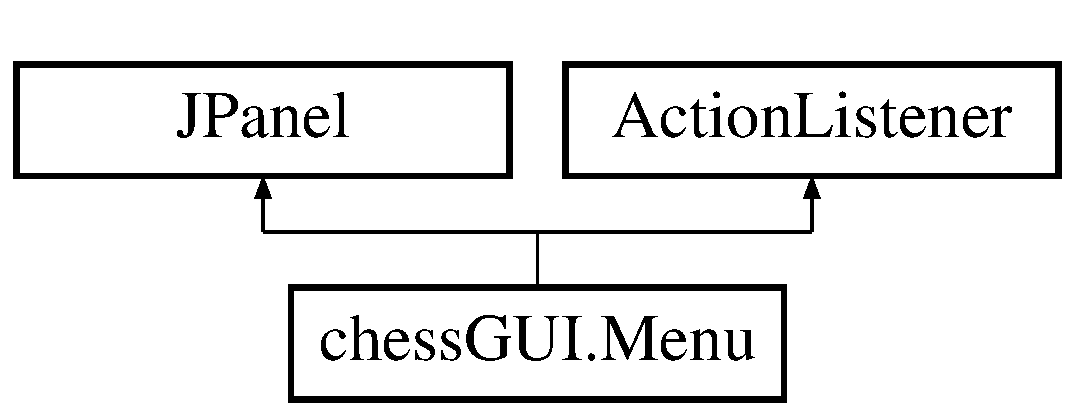
\includegraphics[height=2.000000cm]{classchess_g_u_i_1_1_menu}
\end{center}
\end{figure}
\subsection*{Public Member Functions}
\begin{DoxyCompactItemize}
\item 
\mbox{\Hypertarget{classchess_g_u_i_1_1_menu_acb80a86cb0dd08e2fdcb107568be3102}\label{classchess_g_u_i_1_1_menu_acb80a86cb0dd08e2fdcb107568be3102}} 
void {\bfseries action\+Performed} (Action\+Event e)
\end{DoxyCompactItemize}


The documentation for this class was generated from the following file\+:\begin{DoxyCompactItemize}
\item 
src/chess\+G\+U\+I/Menu.\+java\end{DoxyCompactItemize}

\hypertarget{classchess_build_1_1_pawn}{}\section{chess\+Build.\+Pawn Class Reference}
\label{classchess_build_1_1_pawn}\index{chess\+Build.\+Pawn@{chess\+Build.\+Pawn}}
Inheritance diagram for chess\+Build.\+Pawn\+:\begin{figure}[H]
\begin{center}
\leavevmode
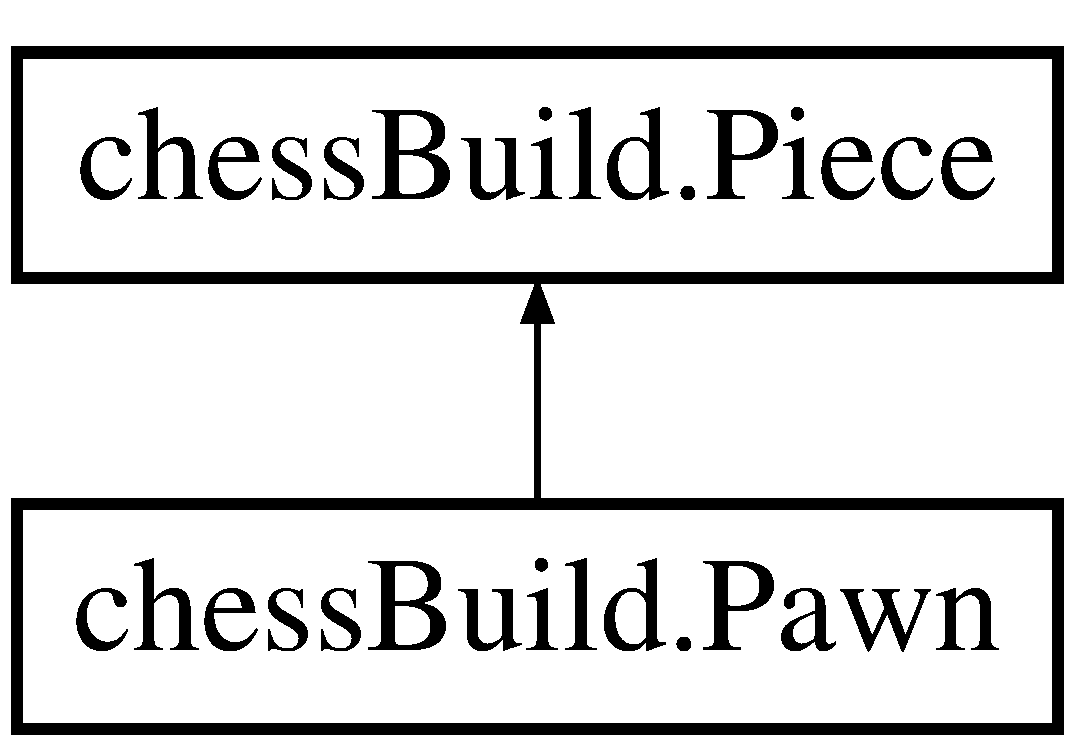
\includegraphics[height=2.000000cm]{classchess_build_1_1_pawn}
\end{center}
\end{figure}
\subsection*{Public Member Functions}
\begin{DoxyCompactItemize}
\item 
\hyperlink{classchess_build_1_1_pawn_abe5ab01673eafb544f5cd3c84a73732d}{Pawn} ()
\item 
\hyperlink{classchess_build_1_1_pawn_aaf18709e792d82b09e27325a118d1230}{Pawn} (\hyperlink{classchess_build_1_1_pawn}{Pawn} other)
\item 
\hyperlink{classchess_build_1_1_pawn_a1e0b4fb3d9b21ef747f2ceb9a2438131}{Pawn} (String color)
\item 
\hyperlink{classchess_build_1_1_pawn_adb46f28a04fdd909fadcca6004df07ba}{Pawn} (int x, int y, String color, boolean is\+Alive)
\item 
\mbox{\Hypertarget{classchess_build_1_1_pawn_a003a68c18a31adf0988dd09a8ffe7aa8}\label{classchess_build_1_1_pawn_a003a68c18a31adf0988dd09a8ffe7aa8}} 
boolean {\bfseries check\+Move} (\hyperlink{classchess_build_1_1_board}{Board} board, int targetX, int targetY)
\end{DoxyCompactItemize}


\subsection{Constructor \& Destructor Documentation}
\mbox{\Hypertarget{classchess_build_1_1_pawn_abe5ab01673eafb544f5cd3c84a73732d}\label{classchess_build_1_1_pawn_abe5ab01673eafb544f5cd3c84a73732d}} 
\index{chess\+Build\+::\+Pawn@{chess\+Build\+::\+Pawn}!Pawn@{Pawn}}
\index{Pawn@{Pawn}!chess\+Build\+::\+Pawn@{chess\+Build\+::\+Pawn}}
\subsubsection{\texorpdfstring{Pawn()}{Pawn()}\hspace{0.1cm}{\footnotesize\ttfamily [1/4]}}
{\footnotesize\ttfamily chess\+Build.\+Pawn.\+Pawn (\begin{DoxyParamCaption}{ }\end{DoxyParamCaption})}

Default Constructor \mbox{\Hypertarget{classchess_build_1_1_pawn_aaf18709e792d82b09e27325a118d1230}\label{classchess_build_1_1_pawn_aaf18709e792d82b09e27325a118d1230}} 
\index{chess\+Build\+::\+Pawn@{chess\+Build\+::\+Pawn}!Pawn@{Pawn}}
\index{Pawn@{Pawn}!chess\+Build\+::\+Pawn@{chess\+Build\+::\+Pawn}}
\subsubsection{\texorpdfstring{Pawn()}{Pawn()}\hspace{0.1cm}{\footnotesize\ttfamily [2/4]}}
{\footnotesize\ttfamily chess\+Build.\+Pawn.\+Pawn (\begin{DoxyParamCaption}\item[{\hyperlink{classchess_build_1_1_pawn}{Pawn}}]{other }\end{DoxyParamCaption})}

Copy constructor 
\begin{DoxyParams}{Parameters}
{\em other} & \\
\hline
\end{DoxyParams}
\mbox{\Hypertarget{classchess_build_1_1_pawn_a1e0b4fb3d9b21ef747f2ceb9a2438131}\label{classchess_build_1_1_pawn_a1e0b4fb3d9b21ef747f2ceb9a2438131}} 
\index{chess\+Build\+::\+Pawn@{chess\+Build\+::\+Pawn}!Pawn@{Pawn}}
\index{Pawn@{Pawn}!chess\+Build\+::\+Pawn@{chess\+Build\+::\+Pawn}}
\subsubsection{\texorpdfstring{Pawn()}{Pawn()}\hspace{0.1cm}{\footnotesize\ttfamily [3/4]}}
{\footnotesize\ttfamily chess\+Build.\+Pawn.\+Pawn (\begin{DoxyParamCaption}\item[{String}]{color }\end{DoxyParamCaption})}

\hyperlink{classchess_build_1_1_pawn}{Pawn} constructor 
\begin{DoxyParams}{Parameters}
{\em color} & \\
\hline
\end{DoxyParams}
\mbox{\Hypertarget{classchess_build_1_1_pawn_adb46f28a04fdd909fadcca6004df07ba}\label{classchess_build_1_1_pawn_adb46f28a04fdd909fadcca6004df07ba}} 
\index{chess\+Build\+::\+Pawn@{chess\+Build\+::\+Pawn}!Pawn@{Pawn}}
\index{Pawn@{Pawn}!chess\+Build\+::\+Pawn@{chess\+Build\+::\+Pawn}}
\subsubsection{\texorpdfstring{Pawn()}{Pawn()}\hspace{0.1cm}{\footnotesize\ttfamily [4/4]}}
{\footnotesize\ttfamily chess\+Build.\+Pawn.\+Pawn (\begin{DoxyParamCaption}\item[{int}]{x,  }\item[{int}]{y,  }\item[{String}]{color,  }\item[{boolean}]{is\+Alive }\end{DoxyParamCaption})}

\hyperlink{classchess_build_1_1_pawn}{Pawn} constructor 
\begin{DoxyParams}{Parameters}
{\em x} & \\
\hline
{\em y} & \\
\hline
{\em color} & \\
\hline
{\em is\+Alive} & \\
\hline
\end{DoxyParams}


The documentation for this class was generated from the following file\+:\begin{DoxyCompactItemize}
\item 
src/chess\+Build/Pawn.\+java\end{DoxyCompactItemize}

\hypertarget{classchess_build_1_1_piece}{}\section{chess\+Build.\+Piece Class Reference}
\label{classchess_build_1_1_piece}\index{chess\+Build.\+Piece@{chess\+Build.\+Piece}}
Inheritance diagram for chess\+Build.\+Piece\+:\begin{figure}[H]
\begin{center}
\leavevmode
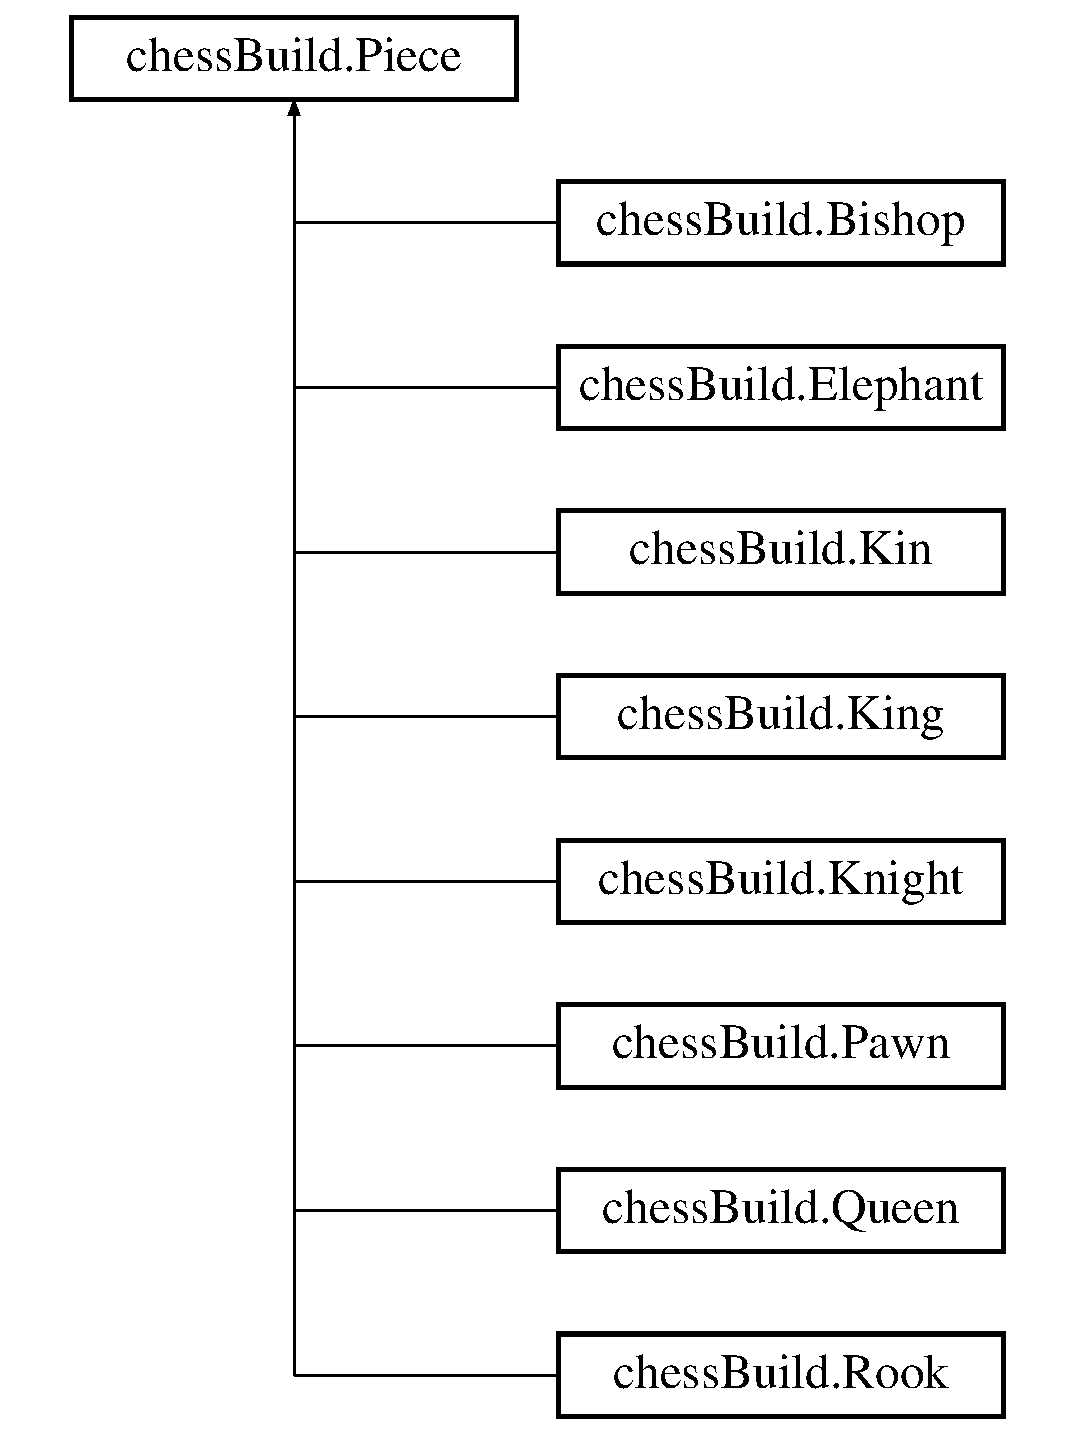
\includegraphics[height=9.000000cm]{classchess_build_1_1_piece}
\end{center}
\end{figure}
\subsection*{Public Member Functions}
\begin{DoxyCompactItemize}
\item 
\hyperlink{classchess_build_1_1_piece_a41b06caa70b1b74ee4adde871cdae1d5}{Piece} ()
\item 
\hyperlink{classchess_build_1_1_piece_ab4cdefaf4be1dcb991257e94227560cf}{Piece} (String color)
\item 
\hyperlink{classchess_build_1_1_piece_a9c0143239c1c8e50aa1a26d13490b816}{Piece} (\hyperlink{classchess_build_1_1_piece}{Piece} other)
\item 
\hyperlink{classchess_build_1_1_piece_a8b3114c959f347293be11e115a0ceada}{Piece} (int x, int y, String color, boolean is\+Alive)
\item 
void \hyperlink{classchess_build_1_1_piece_abcd8667e17514a6dcd27c3bd18e41279}{setX} (int x)
\item 
void \hyperlink{classchess_build_1_1_piece_a3d591027929747d1d2436a702ef15e3d}{setY} (int y)
\item 
void \hyperlink{classchess_build_1_1_piece_a06fc50dacba109b1a3903045f33dd61a}{set\+Color} (String color)
\item 
void \hyperlink{classchess_build_1_1_piece_a15d7482399188a3635f13b11c4a57d1a}{set\+Is\+Alive} (boolean is\+Alive)
\item 
int \hyperlink{classchess_build_1_1_piece_a5d9d98f556141604bbef630597474e42}{getX} ()
\item 
int \hyperlink{classchess_build_1_1_piece_a3c6c4ce7aec8f7c4e802aeee92aa7830}{getY} ()
\item 
String \hyperlink{classchess_build_1_1_piece_a2ed07d6f74a8a36955faad7cbf197348}{get\+Color} ()
\item 
boolean \hyperlink{classchess_build_1_1_piece_a19f95de8f94f11b84a7e1b0a1261825c}{get\+Is\+Alive} ()
\item 
boolean \hyperlink{classchess_build_1_1_piece_a7f4903f049048556c3eb7441259719c0}{check\+Move} (\hyperlink{classchess_build_1_1_board}{Board} board, int targetX, int targetY)
\end{DoxyCompactItemize}


\subsection{Constructor \& Destructor Documentation}
\mbox{\Hypertarget{classchess_build_1_1_piece_a41b06caa70b1b74ee4adde871cdae1d5}\label{classchess_build_1_1_piece_a41b06caa70b1b74ee4adde871cdae1d5}} 
\index{chess\+Build\+::\+Piece@{chess\+Build\+::\+Piece}!Piece@{Piece}}
\index{Piece@{Piece}!chess\+Build\+::\+Piece@{chess\+Build\+::\+Piece}}
\subsubsection{\texorpdfstring{Piece()}{Piece()}\hspace{0.1cm}{\footnotesize\ttfamily [1/4]}}
{\footnotesize\ttfamily chess\+Build.\+Piece.\+Piece (\begin{DoxyParamCaption}{ }\end{DoxyParamCaption})}

Default constructor for piece \mbox{\Hypertarget{classchess_build_1_1_piece_ab4cdefaf4be1dcb991257e94227560cf}\label{classchess_build_1_1_piece_ab4cdefaf4be1dcb991257e94227560cf}} 
\index{chess\+Build\+::\+Piece@{chess\+Build\+::\+Piece}!Piece@{Piece}}
\index{Piece@{Piece}!chess\+Build\+::\+Piece@{chess\+Build\+::\+Piece}}
\subsubsection{\texorpdfstring{Piece()}{Piece()}\hspace{0.1cm}{\footnotesize\ttfamily [2/4]}}
{\footnotesize\ttfamily chess\+Build.\+Piece.\+Piece (\begin{DoxyParamCaption}\item[{String}]{color }\end{DoxyParamCaption})}

Constructor for piece 
\begin{DoxyParams}{Parameters}
{\em color} & \\
\hline
\end{DoxyParams}
\mbox{\Hypertarget{classchess_build_1_1_piece_a9c0143239c1c8e50aa1a26d13490b816}\label{classchess_build_1_1_piece_a9c0143239c1c8e50aa1a26d13490b816}} 
\index{chess\+Build\+::\+Piece@{chess\+Build\+::\+Piece}!Piece@{Piece}}
\index{Piece@{Piece}!chess\+Build\+::\+Piece@{chess\+Build\+::\+Piece}}
\subsubsection{\texorpdfstring{Piece()}{Piece()}\hspace{0.1cm}{\footnotesize\ttfamily [3/4]}}
{\footnotesize\ttfamily chess\+Build.\+Piece.\+Piece (\begin{DoxyParamCaption}\item[{\hyperlink{classchess_build_1_1_piece}{Piece}}]{other }\end{DoxyParamCaption})}

Copy constructor 
\begin{DoxyParams}{Parameters}
{\em other} & \\
\hline
\end{DoxyParams}
\mbox{\Hypertarget{classchess_build_1_1_piece_a8b3114c959f347293be11e115a0ceada}\label{classchess_build_1_1_piece_a8b3114c959f347293be11e115a0ceada}} 
\index{chess\+Build\+::\+Piece@{chess\+Build\+::\+Piece}!Piece@{Piece}}
\index{Piece@{Piece}!chess\+Build\+::\+Piece@{chess\+Build\+::\+Piece}}
\subsubsection{\texorpdfstring{Piece()}{Piece()}\hspace{0.1cm}{\footnotesize\ttfamily [4/4]}}
{\footnotesize\ttfamily chess\+Build.\+Piece.\+Piece (\begin{DoxyParamCaption}\item[{int}]{x,  }\item[{int}]{y,  }\item[{String}]{color,  }\item[{boolean}]{is\+Alive }\end{DoxyParamCaption})}

Constructor for piece 
\begin{DoxyParams}{Parameters}
{\em x} & \\
\hline
{\em y} & \\
\hline
{\em color} & \\
\hline
{\em is\+Alive} & \\
\hline
\end{DoxyParams}


\subsection{Member Function Documentation}
\mbox{\Hypertarget{classchess_build_1_1_piece_a7f4903f049048556c3eb7441259719c0}\label{classchess_build_1_1_piece_a7f4903f049048556c3eb7441259719c0}} 
\index{chess\+Build\+::\+Piece@{chess\+Build\+::\+Piece}!check\+Move@{check\+Move}}
\index{check\+Move@{check\+Move}!chess\+Build\+::\+Piece@{chess\+Build\+::\+Piece}}
\subsubsection{\texorpdfstring{check\+Move()}{checkMove()}}
{\footnotesize\ttfamily boolean chess\+Build.\+Piece.\+check\+Move (\begin{DoxyParamCaption}\item[{\hyperlink{classchess_build_1_1_board}{Board}}]{board,  }\item[{int}]{targetX,  }\item[{int}]{targetY }\end{DoxyParamCaption})}

check\+Move method for piece check whether the piece is out of boundary 
\begin{DoxyParams}{Parameters}
{\em board} & \\
\hline
{\em targetX} & \\
\hline
{\em targetY} & \\
\hline
\end{DoxyParams}
\begin{DoxyReturn}{Returns}

\end{DoxyReturn}
\mbox{\Hypertarget{classchess_build_1_1_piece_a2ed07d6f74a8a36955faad7cbf197348}\label{classchess_build_1_1_piece_a2ed07d6f74a8a36955faad7cbf197348}} 
\index{chess\+Build\+::\+Piece@{chess\+Build\+::\+Piece}!get\+Color@{get\+Color}}
\index{get\+Color@{get\+Color}!chess\+Build\+::\+Piece@{chess\+Build\+::\+Piece}}
\subsubsection{\texorpdfstring{get\+Color()}{getColor()}}
{\footnotesize\ttfamily String chess\+Build.\+Piece.\+get\+Color (\begin{DoxyParamCaption}{ }\end{DoxyParamCaption})}

get color of piece \begin{DoxyReturn}{Returns}

\end{DoxyReturn}
\mbox{\Hypertarget{classchess_build_1_1_piece_a19f95de8f94f11b84a7e1b0a1261825c}\label{classchess_build_1_1_piece_a19f95de8f94f11b84a7e1b0a1261825c}} 
\index{chess\+Build\+::\+Piece@{chess\+Build\+::\+Piece}!get\+Is\+Alive@{get\+Is\+Alive}}
\index{get\+Is\+Alive@{get\+Is\+Alive}!chess\+Build\+::\+Piece@{chess\+Build\+::\+Piece}}
\subsubsection{\texorpdfstring{get\+Is\+Alive()}{getIsAlive()}}
{\footnotesize\ttfamily boolean chess\+Build.\+Piece.\+get\+Is\+Alive (\begin{DoxyParamCaption}{ }\end{DoxyParamCaption})}

get is\+Alive of piece \begin{DoxyReturn}{Returns}

\end{DoxyReturn}
\mbox{\Hypertarget{classchess_build_1_1_piece_a5d9d98f556141604bbef630597474e42}\label{classchess_build_1_1_piece_a5d9d98f556141604bbef630597474e42}} 
\index{chess\+Build\+::\+Piece@{chess\+Build\+::\+Piece}!getX@{getX}}
\index{getX@{getX}!chess\+Build\+::\+Piece@{chess\+Build\+::\+Piece}}
\subsubsection{\texorpdfstring{get\+X()}{getX()}}
{\footnotesize\ttfamily int chess\+Build.\+Piece.\+getX (\begin{DoxyParamCaption}{ }\end{DoxyParamCaption})}

get x of piece \begin{DoxyReturn}{Returns}

\end{DoxyReturn}
\mbox{\Hypertarget{classchess_build_1_1_piece_a3c6c4ce7aec8f7c4e802aeee92aa7830}\label{classchess_build_1_1_piece_a3c6c4ce7aec8f7c4e802aeee92aa7830}} 
\index{chess\+Build\+::\+Piece@{chess\+Build\+::\+Piece}!getY@{getY}}
\index{getY@{getY}!chess\+Build\+::\+Piece@{chess\+Build\+::\+Piece}}
\subsubsection{\texorpdfstring{get\+Y()}{getY()}}
{\footnotesize\ttfamily int chess\+Build.\+Piece.\+getY (\begin{DoxyParamCaption}{ }\end{DoxyParamCaption})}

get y of piece \begin{DoxyReturn}{Returns}

\end{DoxyReturn}
\mbox{\Hypertarget{classchess_build_1_1_piece_a06fc50dacba109b1a3903045f33dd61a}\label{classchess_build_1_1_piece_a06fc50dacba109b1a3903045f33dd61a}} 
\index{chess\+Build\+::\+Piece@{chess\+Build\+::\+Piece}!set\+Color@{set\+Color}}
\index{set\+Color@{set\+Color}!chess\+Build\+::\+Piece@{chess\+Build\+::\+Piece}}
\subsubsection{\texorpdfstring{set\+Color()}{setColor()}}
{\footnotesize\ttfamily void chess\+Build.\+Piece.\+set\+Color (\begin{DoxyParamCaption}\item[{String}]{color }\end{DoxyParamCaption})}

Set color of piece 
\begin{DoxyParams}{Parameters}
{\em color} & \\
\hline
\end{DoxyParams}
\mbox{\Hypertarget{classchess_build_1_1_piece_a15d7482399188a3635f13b11c4a57d1a}\label{classchess_build_1_1_piece_a15d7482399188a3635f13b11c4a57d1a}} 
\index{chess\+Build\+::\+Piece@{chess\+Build\+::\+Piece}!set\+Is\+Alive@{set\+Is\+Alive}}
\index{set\+Is\+Alive@{set\+Is\+Alive}!chess\+Build\+::\+Piece@{chess\+Build\+::\+Piece}}
\subsubsection{\texorpdfstring{set\+Is\+Alive()}{setIsAlive()}}
{\footnotesize\ttfamily void chess\+Build.\+Piece.\+set\+Is\+Alive (\begin{DoxyParamCaption}\item[{boolean}]{is\+Alive }\end{DoxyParamCaption})}

Set is\+Alive of piece 
\begin{DoxyParams}{Parameters}
{\em is\+Alive} & \\
\hline
\end{DoxyParams}
\mbox{\Hypertarget{classchess_build_1_1_piece_abcd8667e17514a6dcd27c3bd18e41279}\label{classchess_build_1_1_piece_abcd8667e17514a6dcd27c3bd18e41279}} 
\index{chess\+Build\+::\+Piece@{chess\+Build\+::\+Piece}!setX@{setX}}
\index{setX@{setX}!chess\+Build\+::\+Piece@{chess\+Build\+::\+Piece}}
\subsubsection{\texorpdfstring{set\+X()}{setX()}}
{\footnotesize\ttfamily void chess\+Build.\+Piece.\+setX (\begin{DoxyParamCaption}\item[{int}]{x }\end{DoxyParamCaption})}

Set x coordinate of piece 
\begin{DoxyParams}{Parameters}
{\em x} & \\
\hline
\end{DoxyParams}
\mbox{\Hypertarget{classchess_build_1_1_piece_a3d591027929747d1d2436a702ef15e3d}\label{classchess_build_1_1_piece_a3d591027929747d1d2436a702ef15e3d}} 
\index{chess\+Build\+::\+Piece@{chess\+Build\+::\+Piece}!setY@{setY}}
\index{setY@{setY}!chess\+Build\+::\+Piece@{chess\+Build\+::\+Piece}}
\subsubsection{\texorpdfstring{set\+Y()}{setY()}}
{\footnotesize\ttfamily void chess\+Build.\+Piece.\+setY (\begin{DoxyParamCaption}\item[{int}]{y }\end{DoxyParamCaption})}

Set y coordinate of piece 
\begin{DoxyParams}{Parameters}
{\em y} & \\
\hline
\end{DoxyParams}


The documentation for this class was generated from the following file\+:\begin{DoxyCompactItemize}
\item 
src/chess\+Build/Piece.\+java\end{DoxyCompactItemize}

\hypertarget{classchess_build_1_1_player}{}\section{chess\+Build.\+Player Class Reference}
\label{classchess_build_1_1_player}\index{chess\+Build.\+Player@{chess\+Build.\+Player}}
\subsection*{Public Member Functions}
\begin{DoxyCompactItemize}
\item 
\hyperlink{classchess_build_1_1_player_af6d8214f5ad0c21e5801c920aa1449db}{Player} (String color)
\item 
\hyperlink{classchess_build_1_1_player_a427c6aeab40552829c8d387b8908c1a1}{Player} (\hyperlink{classchess_build_1_1_player}{Player} other)
\item 
void \hyperlink{classchess_build_1_1_player_abc3aee1d3b1ce4ab0a12d2c544cc7e08}{set\+Color} (String color)
\item 
String \hyperlink{classchess_build_1_1_player_a2d04858909da7c3313939ab657c7541b}{get\+Color} ()
\item 
Array\+List$<$ \hyperlink{classchess_build_1_1_pawn}{Pawn} $>$ \hyperlink{classchess_build_1_1_player_a031a92644a92ed146404db4332f76303}{get\+Track\+Pawn} ()
\item 
Array\+List$<$ \hyperlink{classchess_build_1_1_knight}{Knight} $>$ \hyperlink{classchess_build_1_1_player_af50e14cc2f948a18460bb09278c44016}{get\+Track\+Knight} ()
\item 
Array\+List$<$ \hyperlink{classchess_build_1_1_bishop}{Bishop} $>$ \hyperlink{classchess_build_1_1_player_a381227f722157384cbd9fa1730374e09}{get\+Track\+Bishop} ()
\item 
Array\+List$<$ \hyperlink{classchess_build_1_1_rook}{Rook} $>$ \hyperlink{classchess_build_1_1_player_a24e07f2fb2000ac07bc7e350b7ba5715}{get\+Track\+Rook} ()
\item 
Array\+List$<$ \hyperlink{classchess_build_1_1_queen}{Queen} $>$ \hyperlink{classchess_build_1_1_player_aef2b846009857d7387fdcbf28b111338}{get\+Track\+Queen} ()
\item 
Array\+List$<$ \hyperlink{classchess_build_1_1_king}{King} $>$ \hyperlink{classchess_build_1_1_player_a62347626dff2ff6a2e63d33b4bcb5174}{get\+Track\+King} ()
\item 
Array\+List$<$ \hyperlink{classchess_build_1_1_kin}{Kin} $>$ \hyperlink{classchess_build_1_1_player_aed6e29a8e82ce3ae654b1773cb403cf3}{get\+Track\+Kin} ()
\item 
Array\+List$<$ \hyperlink{classchess_build_1_1_elephant}{Elephant} $>$ \hyperlink{classchess_build_1_1_player_ad45b47c46c9940e067b7d23f765ed2ce}{get\+Track\+Elephant} ()
\end{DoxyCompactItemize}


\subsection{Constructor \& Destructor Documentation}
\mbox{\Hypertarget{classchess_build_1_1_player_af6d8214f5ad0c21e5801c920aa1449db}\label{classchess_build_1_1_player_af6d8214f5ad0c21e5801c920aa1449db}} 
\index{chess\+Build\+::\+Player@{chess\+Build\+::\+Player}!Player@{Player}}
\index{Player@{Player}!chess\+Build\+::\+Player@{chess\+Build\+::\+Player}}
\subsubsection{\texorpdfstring{Player()}{Player()}\hspace{0.1cm}{\footnotesize\ttfamily [1/2]}}
{\footnotesize\ttfamily chess\+Build.\+Player.\+Player (\begin{DoxyParamCaption}\item[{String}]{color }\end{DoxyParamCaption})}

Constructor for player 
\begin{DoxyParams}{Parameters}
{\em color} & \\
\hline
\end{DoxyParams}
\mbox{\Hypertarget{classchess_build_1_1_player_a427c6aeab40552829c8d387b8908c1a1}\label{classchess_build_1_1_player_a427c6aeab40552829c8d387b8908c1a1}} 
\index{chess\+Build\+::\+Player@{chess\+Build\+::\+Player}!Player@{Player}}
\index{Player@{Player}!chess\+Build\+::\+Player@{chess\+Build\+::\+Player}}
\subsubsection{\texorpdfstring{Player()}{Player()}\hspace{0.1cm}{\footnotesize\ttfamily [2/2]}}
{\footnotesize\ttfamily chess\+Build.\+Player.\+Player (\begin{DoxyParamCaption}\item[{\hyperlink{classchess_build_1_1_player}{Player}}]{other }\end{DoxyParamCaption})}

Copy constructor 
\begin{DoxyParams}{Parameters}
{\em other} & \\
\hline
\end{DoxyParams}


\subsection{Member Function Documentation}
\mbox{\Hypertarget{classchess_build_1_1_player_a2d04858909da7c3313939ab657c7541b}\label{classchess_build_1_1_player_a2d04858909da7c3313939ab657c7541b}} 
\index{chess\+Build\+::\+Player@{chess\+Build\+::\+Player}!get\+Color@{get\+Color}}
\index{get\+Color@{get\+Color}!chess\+Build\+::\+Player@{chess\+Build\+::\+Player}}
\subsubsection{\texorpdfstring{get\+Color()}{getColor()}}
{\footnotesize\ttfamily String chess\+Build.\+Player.\+get\+Color (\begin{DoxyParamCaption}{ }\end{DoxyParamCaption})}

Get color method for player \begin{DoxyReturn}{Returns}

\end{DoxyReturn}
\mbox{\Hypertarget{classchess_build_1_1_player_a381227f722157384cbd9fa1730374e09}\label{classchess_build_1_1_player_a381227f722157384cbd9fa1730374e09}} 
\index{chess\+Build\+::\+Player@{chess\+Build\+::\+Player}!get\+Track\+Bishop@{get\+Track\+Bishop}}
\index{get\+Track\+Bishop@{get\+Track\+Bishop}!chess\+Build\+::\+Player@{chess\+Build\+::\+Player}}
\subsubsection{\texorpdfstring{get\+Track\+Bishop()}{getTrackBishop()}}
{\footnotesize\ttfamily Array\+List$<$\hyperlink{classchess_build_1_1_bishop}{Bishop}$>$ chess\+Build.\+Player.\+get\+Track\+Bishop (\begin{DoxyParamCaption}{ }\end{DoxyParamCaption})}

Get\+Track\+Bishop method for player \begin{DoxyReturn}{Returns}

\end{DoxyReturn}
\mbox{\Hypertarget{classchess_build_1_1_player_ad45b47c46c9940e067b7d23f765ed2ce}\label{classchess_build_1_1_player_ad45b47c46c9940e067b7d23f765ed2ce}} 
\index{chess\+Build\+::\+Player@{chess\+Build\+::\+Player}!get\+Track\+Elephant@{get\+Track\+Elephant}}
\index{get\+Track\+Elephant@{get\+Track\+Elephant}!chess\+Build\+::\+Player@{chess\+Build\+::\+Player}}
\subsubsection{\texorpdfstring{get\+Track\+Elephant()}{getTrackElephant()}}
{\footnotesize\ttfamily Array\+List$<$\hyperlink{classchess_build_1_1_elephant}{Elephant}$>$ chess\+Build.\+Player.\+get\+Track\+Elephant (\begin{DoxyParamCaption}{ }\end{DoxyParamCaption})}

Get\+Track\+Elephant for player \begin{DoxyReturn}{Returns}

\end{DoxyReturn}
\mbox{\Hypertarget{classchess_build_1_1_player_aed6e29a8e82ce3ae654b1773cb403cf3}\label{classchess_build_1_1_player_aed6e29a8e82ce3ae654b1773cb403cf3}} 
\index{chess\+Build\+::\+Player@{chess\+Build\+::\+Player}!get\+Track\+Kin@{get\+Track\+Kin}}
\index{get\+Track\+Kin@{get\+Track\+Kin}!chess\+Build\+::\+Player@{chess\+Build\+::\+Player}}
\subsubsection{\texorpdfstring{get\+Track\+Kin()}{getTrackKin()}}
{\footnotesize\ttfamily Array\+List$<$\hyperlink{classchess_build_1_1_kin}{Kin}$>$ chess\+Build.\+Player.\+get\+Track\+Kin (\begin{DoxyParamCaption}{ }\end{DoxyParamCaption})}

Get\+Track\+Kin for player \begin{DoxyReturn}{Returns}

\end{DoxyReturn}
\mbox{\Hypertarget{classchess_build_1_1_player_a62347626dff2ff6a2e63d33b4bcb5174}\label{classchess_build_1_1_player_a62347626dff2ff6a2e63d33b4bcb5174}} 
\index{chess\+Build\+::\+Player@{chess\+Build\+::\+Player}!get\+Track\+King@{get\+Track\+King}}
\index{get\+Track\+King@{get\+Track\+King}!chess\+Build\+::\+Player@{chess\+Build\+::\+Player}}
\subsubsection{\texorpdfstring{get\+Track\+King()}{getTrackKing()}}
{\footnotesize\ttfamily Array\+List$<$\hyperlink{classchess_build_1_1_king}{King}$>$ chess\+Build.\+Player.\+get\+Track\+King (\begin{DoxyParamCaption}{ }\end{DoxyParamCaption})}

Get\+Track\+King method for player \begin{DoxyReturn}{Returns}

\end{DoxyReturn}
\mbox{\Hypertarget{classchess_build_1_1_player_af50e14cc2f948a18460bb09278c44016}\label{classchess_build_1_1_player_af50e14cc2f948a18460bb09278c44016}} 
\index{chess\+Build\+::\+Player@{chess\+Build\+::\+Player}!get\+Track\+Knight@{get\+Track\+Knight}}
\index{get\+Track\+Knight@{get\+Track\+Knight}!chess\+Build\+::\+Player@{chess\+Build\+::\+Player}}
\subsubsection{\texorpdfstring{get\+Track\+Knight()}{getTrackKnight()}}
{\footnotesize\ttfamily Array\+List$<$\hyperlink{classchess_build_1_1_knight}{Knight}$>$ chess\+Build.\+Player.\+get\+Track\+Knight (\begin{DoxyParamCaption}{ }\end{DoxyParamCaption})}

Get\+Track\+Knight method for player \begin{DoxyReturn}{Returns}

\end{DoxyReturn}
\mbox{\Hypertarget{classchess_build_1_1_player_a031a92644a92ed146404db4332f76303}\label{classchess_build_1_1_player_a031a92644a92ed146404db4332f76303}} 
\index{chess\+Build\+::\+Player@{chess\+Build\+::\+Player}!get\+Track\+Pawn@{get\+Track\+Pawn}}
\index{get\+Track\+Pawn@{get\+Track\+Pawn}!chess\+Build\+::\+Player@{chess\+Build\+::\+Player}}
\subsubsection{\texorpdfstring{get\+Track\+Pawn()}{getTrackPawn()}}
{\footnotesize\ttfamily Array\+List$<$\hyperlink{classchess_build_1_1_pawn}{Pawn}$>$ chess\+Build.\+Player.\+get\+Track\+Pawn (\begin{DoxyParamCaption}{ }\end{DoxyParamCaption})}

Get\+Track\+Pawn method for player \begin{DoxyReturn}{Returns}

\end{DoxyReturn}
\mbox{\Hypertarget{classchess_build_1_1_player_aef2b846009857d7387fdcbf28b111338}\label{classchess_build_1_1_player_aef2b846009857d7387fdcbf28b111338}} 
\index{chess\+Build\+::\+Player@{chess\+Build\+::\+Player}!get\+Track\+Queen@{get\+Track\+Queen}}
\index{get\+Track\+Queen@{get\+Track\+Queen}!chess\+Build\+::\+Player@{chess\+Build\+::\+Player}}
\subsubsection{\texorpdfstring{get\+Track\+Queen()}{getTrackQueen()}}
{\footnotesize\ttfamily Array\+List$<$\hyperlink{classchess_build_1_1_queen}{Queen}$>$ chess\+Build.\+Player.\+get\+Track\+Queen (\begin{DoxyParamCaption}{ }\end{DoxyParamCaption})}

Get\+Track\+Queen method for player \begin{DoxyReturn}{Returns}

\end{DoxyReturn}
\mbox{\Hypertarget{classchess_build_1_1_player_a24e07f2fb2000ac07bc7e350b7ba5715}\label{classchess_build_1_1_player_a24e07f2fb2000ac07bc7e350b7ba5715}} 
\index{chess\+Build\+::\+Player@{chess\+Build\+::\+Player}!get\+Track\+Rook@{get\+Track\+Rook}}
\index{get\+Track\+Rook@{get\+Track\+Rook}!chess\+Build\+::\+Player@{chess\+Build\+::\+Player}}
\subsubsection{\texorpdfstring{get\+Track\+Rook()}{getTrackRook()}}
{\footnotesize\ttfamily Array\+List$<$\hyperlink{classchess_build_1_1_rook}{Rook}$>$ chess\+Build.\+Player.\+get\+Track\+Rook (\begin{DoxyParamCaption}{ }\end{DoxyParamCaption})}

Get\+Track\+Rook method for player \begin{DoxyReturn}{Returns}

\end{DoxyReturn}
\mbox{\Hypertarget{classchess_build_1_1_player_abc3aee1d3b1ce4ab0a12d2c544cc7e08}\label{classchess_build_1_1_player_abc3aee1d3b1ce4ab0a12d2c544cc7e08}} 
\index{chess\+Build\+::\+Player@{chess\+Build\+::\+Player}!set\+Color@{set\+Color}}
\index{set\+Color@{set\+Color}!chess\+Build\+::\+Player@{chess\+Build\+::\+Player}}
\subsubsection{\texorpdfstring{set\+Color()}{setColor()}}
{\footnotesize\ttfamily void chess\+Build.\+Player.\+set\+Color (\begin{DoxyParamCaption}\item[{String}]{color }\end{DoxyParamCaption})}

Set color methods for player 
\begin{DoxyParams}{Parameters}
{\em color} & \\
\hline
\end{DoxyParams}


The documentation for this class was generated from the following file\+:\begin{DoxyCompactItemize}
\item 
src/chess\+Build/Player.\+java\end{DoxyCompactItemize}

\hypertarget{classchess_build_1_1_queen}{}\section{chess\+Build.\+Queen Class Reference}
\label{classchess_build_1_1_queen}\index{chess\+Build.\+Queen@{chess\+Build.\+Queen}}
Inheritance diagram for chess\+Build.\+Queen\+:\begin{figure}[H]
\begin{center}
\leavevmode
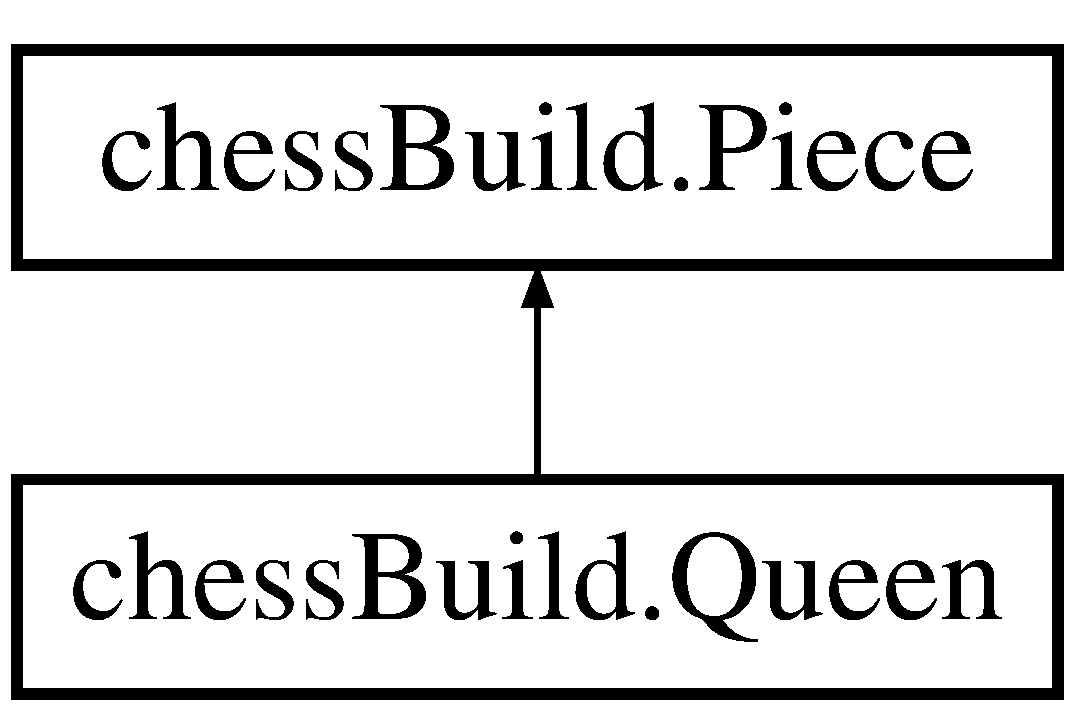
\includegraphics[height=2.000000cm]{classchess_build_1_1_queen}
\end{center}
\end{figure}
\subsection*{Public Member Functions}
\begin{DoxyCompactItemize}
\item 
\hyperlink{classchess_build_1_1_queen_a658925f2dd8632546a22d67ff1a8c4bf}{Queen} ()
\item 
\hyperlink{classchess_build_1_1_queen_a6569f23986b77bf85faeac5f15661a6c}{Queen} (\hyperlink{classchess_build_1_1_queen}{Queen} other)
\item 
\hyperlink{classchess_build_1_1_queen_a142d6ff4a3adb06f4594d0e91549ad92}{Queen} (String color)
\item 
\hyperlink{classchess_build_1_1_queen_a205a888b7cd5393711634e4e6f39fe5e}{Queen} (int x, int y, String color, boolean is\+Alive)
\item 
\mbox{\Hypertarget{classchess_build_1_1_queen_aba9cbeff1f0aed91f0dcf1373d13efca}\label{classchess_build_1_1_queen_aba9cbeff1f0aed91f0dcf1373d13efca}} 
boolean {\bfseries check\+Move} (\hyperlink{classchess_build_1_1_board}{Board} board, int targetX, int targetY)
\item 
boolean \hyperlink{classchess_build_1_1_queen_ab08d98e2b32cfcc4095b468aa9d7248e}{check\+Queen\+Move\+Helper} (\hyperlink{classchess_build_1_1_board}{Board} board, int targetX, int targetY)
\end{DoxyCompactItemize}


\subsection{Constructor \& Destructor Documentation}
\mbox{\Hypertarget{classchess_build_1_1_queen_a658925f2dd8632546a22d67ff1a8c4bf}\label{classchess_build_1_1_queen_a658925f2dd8632546a22d67ff1a8c4bf}} 
\index{chess\+Build\+::\+Queen@{chess\+Build\+::\+Queen}!Queen@{Queen}}
\index{Queen@{Queen}!chess\+Build\+::\+Queen@{chess\+Build\+::\+Queen}}
\subsubsection{\texorpdfstring{Queen()}{Queen()}\hspace{0.1cm}{\footnotesize\ttfamily [1/4]}}
{\footnotesize\ttfamily chess\+Build.\+Queen.\+Queen (\begin{DoxyParamCaption}{ }\end{DoxyParamCaption})}

Default constructor \mbox{\Hypertarget{classchess_build_1_1_queen_a6569f23986b77bf85faeac5f15661a6c}\label{classchess_build_1_1_queen_a6569f23986b77bf85faeac5f15661a6c}} 
\index{chess\+Build\+::\+Queen@{chess\+Build\+::\+Queen}!Queen@{Queen}}
\index{Queen@{Queen}!chess\+Build\+::\+Queen@{chess\+Build\+::\+Queen}}
\subsubsection{\texorpdfstring{Queen()}{Queen()}\hspace{0.1cm}{\footnotesize\ttfamily [2/4]}}
{\footnotesize\ttfamily chess\+Build.\+Queen.\+Queen (\begin{DoxyParamCaption}\item[{\hyperlink{classchess_build_1_1_queen}{Queen}}]{other }\end{DoxyParamCaption})}

Copy constructor 
\begin{DoxyParams}{Parameters}
{\em other} & \\
\hline
\end{DoxyParams}
\mbox{\Hypertarget{classchess_build_1_1_queen_a142d6ff4a3adb06f4594d0e91549ad92}\label{classchess_build_1_1_queen_a142d6ff4a3adb06f4594d0e91549ad92}} 
\index{chess\+Build\+::\+Queen@{chess\+Build\+::\+Queen}!Queen@{Queen}}
\index{Queen@{Queen}!chess\+Build\+::\+Queen@{chess\+Build\+::\+Queen}}
\subsubsection{\texorpdfstring{Queen()}{Queen()}\hspace{0.1cm}{\footnotesize\ttfamily [3/4]}}
{\footnotesize\ttfamily chess\+Build.\+Queen.\+Queen (\begin{DoxyParamCaption}\item[{String}]{color }\end{DoxyParamCaption})}

\hyperlink{classchess_build_1_1_queen}{Queen} constructor 
\begin{DoxyParams}{Parameters}
{\em color} & \\
\hline
\end{DoxyParams}
\mbox{\Hypertarget{classchess_build_1_1_queen_a205a888b7cd5393711634e4e6f39fe5e}\label{classchess_build_1_1_queen_a205a888b7cd5393711634e4e6f39fe5e}} 
\index{chess\+Build\+::\+Queen@{chess\+Build\+::\+Queen}!Queen@{Queen}}
\index{Queen@{Queen}!chess\+Build\+::\+Queen@{chess\+Build\+::\+Queen}}
\subsubsection{\texorpdfstring{Queen()}{Queen()}\hspace{0.1cm}{\footnotesize\ttfamily [4/4]}}
{\footnotesize\ttfamily chess\+Build.\+Queen.\+Queen (\begin{DoxyParamCaption}\item[{int}]{x,  }\item[{int}]{y,  }\item[{String}]{color,  }\item[{boolean}]{is\+Alive }\end{DoxyParamCaption})}

\hyperlink{classchess_build_1_1_queen}{Queen} constructor 
\begin{DoxyParams}{Parameters}
{\em x} & \\
\hline
{\em y} & \\
\hline
{\em color} & \\
\hline
{\em is\+Alive} & \\
\hline
\end{DoxyParams}


\subsection{Member Function Documentation}
\mbox{\Hypertarget{classchess_build_1_1_queen_ab08d98e2b32cfcc4095b468aa9d7248e}\label{classchess_build_1_1_queen_ab08d98e2b32cfcc4095b468aa9d7248e}} 
\index{chess\+Build\+::\+Queen@{chess\+Build\+::\+Queen}!check\+Queen\+Move\+Helper@{check\+Queen\+Move\+Helper}}
\index{check\+Queen\+Move\+Helper@{check\+Queen\+Move\+Helper}!chess\+Build\+::\+Queen@{chess\+Build\+::\+Queen}}
\subsubsection{\texorpdfstring{check\+Queen\+Move\+Helper()}{checkQueenMoveHelper()}}
{\footnotesize\ttfamily boolean chess\+Build.\+Queen.\+check\+Queen\+Move\+Helper (\begin{DoxyParamCaption}\item[{\hyperlink{classchess_build_1_1_board}{Board}}]{board,  }\item[{int}]{targetX,  }\item[{int}]{targetY }\end{DoxyParamCaption})}

Helper function for check\+Move 
\begin{DoxyParams}{Parameters}
{\em board} & \\
\hline
{\em targetX} & \\
\hline
{\em targetY} & \\
\hline
\end{DoxyParams}
\begin{DoxyReturn}{Returns}

\end{DoxyReturn}


The documentation for this class was generated from the following file\+:\begin{DoxyCompactItemize}
\item 
src/chess\+Build/Queen.\+java\end{DoxyCompactItemize}

\hypertarget{classchess_build_1_1_rook}{}\section{chess\+Build.\+Rook Class Reference}
\label{classchess_build_1_1_rook}\index{chess\+Build.\+Rook@{chess\+Build.\+Rook}}
Inheritance diagram for chess\+Build.\+Rook\+:\begin{figure}[H]
\begin{center}
\leavevmode
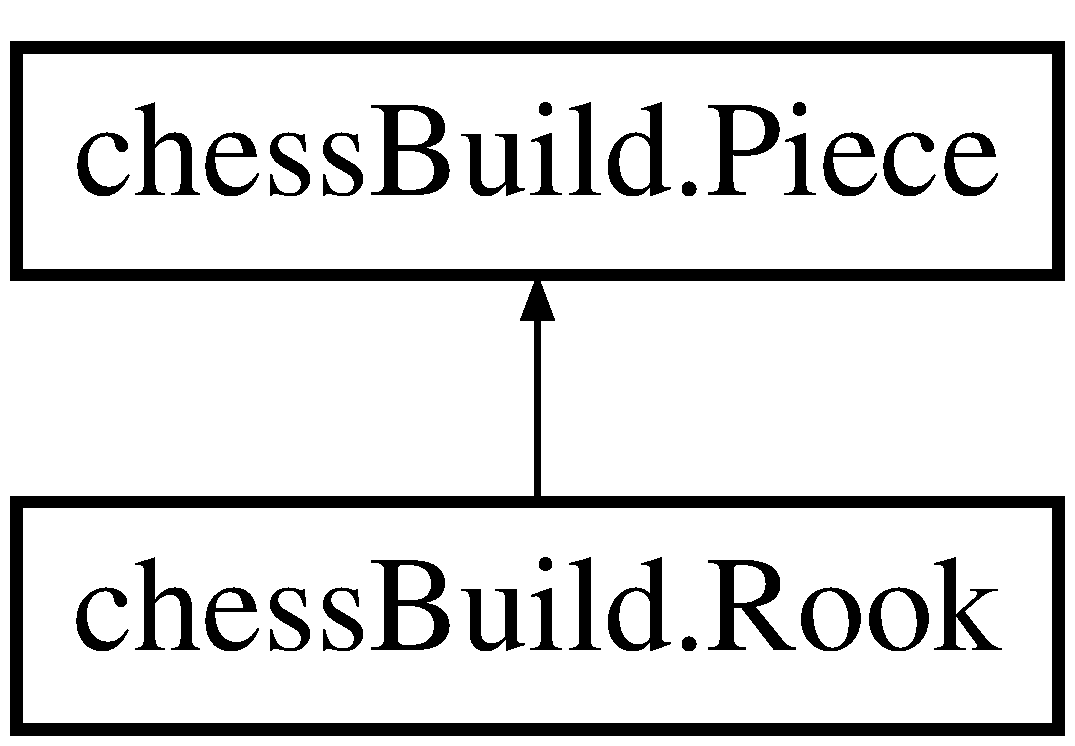
\includegraphics[height=2.000000cm]{classchess_build_1_1_rook}
\end{center}
\end{figure}
\subsection*{Public Member Functions}
\begin{DoxyCompactItemize}
\item 
\hyperlink{classchess_build_1_1_rook_a9967db4000d7beac455338a45ffd43bc}{Rook} ()
\item 
\hyperlink{classchess_build_1_1_rook_a79c81af4e999db11ceb66e8049d33b16}{Rook} (\hyperlink{classchess_build_1_1_rook}{Rook} other)
\item 
\hyperlink{classchess_build_1_1_rook_aff5411564cfd90a16a74290124bbdae3}{Rook} (String color)
\item 
\hyperlink{classchess_build_1_1_rook_a1b2faa9ca40b7fed9172ffe0b15237d9}{Rook} (int x, int y, String color, boolean is\+Alive)
\item 
\mbox{\Hypertarget{classchess_build_1_1_rook_af745f7c175e2ef88983a20db46d22583}\label{classchess_build_1_1_rook_af745f7c175e2ef88983a20db46d22583}} 
boolean {\bfseries check\+Move} (\hyperlink{classchess_build_1_1_board}{Board} board, int targetX, int targetY)
\item 
boolean \hyperlink{classchess_build_1_1_rook_a9d7f5bc7080721398cfd7f0ae3166494}{check\+Rook\+Move\+Helper} (\hyperlink{classchess_build_1_1_board}{Board} board, int targetX, int targetY)
\end{DoxyCompactItemize}


\subsection{Constructor \& Destructor Documentation}
\mbox{\Hypertarget{classchess_build_1_1_rook_a9967db4000d7beac455338a45ffd43bc}\label{classchess_build_1_1_rook_a9967db4000d7beac455338a45ffd43bc}} 
\index{chess\+Build\+::\+Rook@{chess\+Build\+::\+Rook}!Rook@{Rook}}
\index{Rook@{Rook}!chess\+Build\+::\+Rook@{chess\+Build\+::\+Rook}}
\subsubsection{\texorpdfstring{Rook()}{Rook()}\hspace{0.1cm}{\footnotesize\ttfamily [1/4]}}
{\footnotesize\ttfamily chess\+Build.\+Rook.\+Rook (\begin{DoxyParamCaption}{ }\end{DoxyParamCaption})}

Default constructor for rook \mbox{\Hypertarget{classchess_build_1_1_rook_a79c81af4e999db11ceb66e8049d33b16}\label{classchess_build_1_1_rook_a79c81af4e999db11ceb66e8049d33b16}} 
\index{chess\+Build\+::\+Rook@{chess\+Build\+::\+Rook}!Rook@{Rook}}
\index{Rook@{Rook}!chess\+Build\+::\+Rook@{chess\+Build\+::\+Rook}}
\subsubsection{\texorpdfstring{Rook()}{Rook()}\hspace{0.1cm}{\footnotesize\ttfamily [2/4]}}
{\footnotesize\ttfamily chess\+Build.\+Rook.\+Rook (\begin{DoxyParamCaption}\item[{\hyperlink{classchess_build_1_1_rook}{Rook}}]{other }\end{DoxyParamCaption})}

Copy constructor 
\begin{DoxyParams}{Parameters}
{\em other} & \\
\hline
\end{DoxyParams}
\mbox{\Hypertarget{classchess_build_1_1_rook_aff5411564cfd90a16a74290124bbdae3}\label{classchess_build_1_1_rook_aff5411564cfd90a16a74290124bbdae3}} 
\index{chess\+Build\+::\+Rook@{chess\+Build\+::\+Rook}!Rook@{Rook}}
\index{Rook@{Rook}!chess\+Build\+::\+Rook@{chess\+Build\+::\+Rook}}
\subsubsection{\texorpdfstring{Rook()}{Rook()}\hspace{0.1cm}{\footnotesize\ttfamily [3/4]}}
{\footnotesize\ttfamily chess\+Build.\+Rook.\+Rook (\begin{DoxyParamCaption}\item[{String}]{color }\end{DoxyParamCaption})}

\hyperlink{classchess_build_1_1_rook}{Rook} constructor 
\begin{DoxyParams}{Parameters}
{\em color} & \\
\hline
\end{DoxyParams}
\mbox{\Hypertarget{classchess_build_1_1_rook_a1b2faa9ca40b7fed9172ffe0b15237d9}\label{classchess_build_1_1_rook_a1b2faa9ca40b7fed9172ffe0b15237d9}} 
\index{chess\+Build\+::\+Rook@{chess\+Build\+::\+Rook}!Rook@{Rook}}
\index{Rook@{Rook}!chess\+Build\+::\+Rook@{chess\+Build\+::\+Rook}}
\subsubsection{\texorpdfstring{Rook()}{Rook()}\hspace{0.1cm}{\footnotesize\ttfamily [4/4]}}
{\footnotesize\ttfamily chess\+Build.\+Rook.\+Rook (\begin{DoxyParamCaption}\item[{int}]{x,  }\item[{int}]{y,  }\item[{String}]{color,  }\item[{boolean}]{is\+Alive }\end{DoxyParamCaption})}

\hyperlink{classchess_build_1_1_rook}{Rook} constructor 
\begin{DoxyParams}{Parameters}
{\em x} & \\
\hline
{\em y} & \\
\hline
{\em color} & \\
\hline
{\em is\+Alive} & \\
\hline
\end{DoxyParams}


\subsection{Member Function Documentation}
\mbox{\Hypertarget{classchess_build_1_1_rook_a9d7f5bc7080721398cfd7f0ae3166494}\label{classchess_build_1_1_rook_a9d7f5bc7080721398cfd7f0ae3166494}} 
\index{chess\+Build\+::\+Rook@{chess\+Build\+::\+Rook}!check\+Rook\+Move\+Helper@{check\+Rook\+Move\+Helper}}
\index{check\+Rook\+Move\+Helper@{check\+Rook\+Move\+Helper}!chess\+Build\+::\+Rook@{chess\+Build\+::\+Rook}}
\subsubsection{\texorpdfstring{check\+Rook\+Move\+Helper()}{checkRookMoveHelper()}}
{\footnotesize\ttfamily boolean chess\+Build.\+Rook.\+check\+Rook\+Move\+Helper (\begin{DoxyParamCaption}\item[{\hyperlink{classchess_build_1_1_board}{Board}}]{board,  }\item[{int}]{targetX,  }\item[{int}]{targetY }\end{DoxyParamCaption})}

Helper function for check\+Move method 
\begin{DoxyParams}{Parameters}
{\em board} & \\
\hline
{\em targetX} & \\
\hline
{\em targetY} & \\
\hline
\end{DoxyParams}
\begin{DoxyReturn}{Returns}

\end{DoxyReturn}


The documentation for this class was generated from the following file\+:\begin{DoxyCompactItemize}
\item 
src/chess\+Build/Rook.\+java\end{DoxyCompactItemize}

\hypertarget{class_tests_1_1test_bishop}{}\section{Tests.\+test\+Bishop Class Reference}
\label{class_tests_1_1test_bishop}\index{Tests.\+test\+Bishop@{Tests.\+test\+Bishop}}
\subsection*{Public Member Functions}
\begin{DoxyCompactItemize}
\item 
\mbox{\Hypertarget{class_tests_1_1test_bishop_a00afd1a97ca4a83ce359504d1ffd5871}\label{class_tests_1_1test_bishop_a00afd1a97ca4a83ce359504d1ffd5871}} 
void {\bfseries test\+Bishop\+Position} ()  throws Exception
\item 
\mbox{\Hypertarget{class_tests_1_1test_bishop_a2caa9a47ad66c8f79d4e01015791582c}\label{class_tests_1_1test_bishop_a2caa9a47ad66c8f79d4e01015791582c}} 
void {\bfseries test\+Bishop\+Move} ()  throws Exception
\end{DoxyCompactItemize}


The documentation for this class was generated from the following file\+:\begin{DoxyCompactItemize}
\item 
src/\+Tests/test\+Bishop.\+java\end{DoxyCompactItemize}

\hypertarget{class_tests_1_1test_board}{}\section{Tests.\+test\+Board Class Reference}
\label{class_tests_1_1test_board}\index{Tests.\+test\+Board@{Tests.\+test\+Board}}


The documentation for this class was generated from the following file\+:\begin{DoxyCompactItemize}
\item 
src/\+Tests/test\+Board.\+java\end{DoxyCompactItemize}

\hypertarget{class_tests_1_1test_elephant}{}\section{Tests.\+test\+Elephant Class Reference}
\label{class_tests_1_1test_elephant}\index{Tests.\+test\+Elephant@{Tests.\+test\+Elephant}}
\subsection*{Public Member Functions}
\begin{DoxyCompactItemize}
\item 
\mbox{\Hypertarget{class_tests_1_1test_elephant_a7f479921fb60b6cce8a6f710f9543999}\label{class_tests_1_1test_elephant_a7f479921fb60b6cce8a6f710f9543999}} 
void {\bfseries test\+Elephant\+Move} ()  throws Exception
\item 
\mbox{\Hypertarget{class_tests_1_1test_elephant_a812f0993b146a922964214b7c2792cce}\label{class_tests_1_1test_elephant_a812f0993b146a922964214b7c2792cce}} 
void {\bfseries test\+Elephant\+Eat\+Piece} ()  throws Exception
\end{DoxyCompactItemize}


The documentation for this class was generated from the following file\+:\begin{DoxyCompactItemize}
\item 
src/\+Tests/test\+Elephant.\+java\end{DoxyCompactItemize}

\hypertarget{class_tests_1_1test_game}{}\section{Tests.\+test\+Game Class Reference}
\label{class_tests_1_1test_game}\index{Tests.\+test\+Game@{Tests.\+test\+Game}}
\subsection*{Public Member Functions}
\begin{DoxyCompactItemize}
\item 
\mbox{\Hypertarget{class_tests_1_1test_game_ac2ea48c2e0a3c2da0c50340add120907}\label{class_tests_1_1test_game_ac2ea48c2e0a3c2da0c50340add120907}} 
void {\bfseries test\+Game\+Initialize} ()  throws Exception
\item 
\mbox{\Hypertarget{class_tests_1_1test_game_ad254bc120efed7ce38f702fc6123bbb8}\label{class_tests_1_1test_game_ad254bc120efed7ce38f702fc6123bbb8}} 
void {\bfseries test\+Piece\+Move} ()  throws Exception
\item 
\mbox{\Hypertarget{class_tests_1_1test_game_af31c7fa0777baeb91b7a13a8ed8949eb}\label{class_tests_1_1test_game_af31c7fa0777baeb91b7a13a8ed8949eb}} 
void {\bfseries test\+Check\+Mate} ()
\item 
\mbox{\Hypertarget{class_tests_1_1test_game_a3faa83edd4ec3e4ba1f4d9d26434827f}\label{class_tests_1_1test_game_a3faa83edd4ec3e4ba1f4d9d26434827f}} 
void {\bfseries test\+Game\+Winner} ()  throws Exception
\end{DoxyCompactItemize}


The documentation for this class was generated from the following file\+:\begin{DoxyCompactItemize}
\item 
src/\+Tests/test\+Game.\+java\end{DoxyCompactItemize}

\hypertarget{class_tests_1_1test_kin}{}\section{Tests.\+test\+Kin Class Reference}
\label{class_tests_1_1test_kin}\index{Tests.\+test\+Kin@{Tests.\+test\+Kin}}
\subsection*{Public Member Functions}
\begin{DoxyCompactItemize}
\item 
\mbox{\Hypertarget{class_tests_1_1test_kin_a16d9c789050f127072276d041617d3ac}\label{class_tests_1_1test_kin_a16d9c789050f127072276d041617d3ac}} 
void {\bfseries test\+Kin\+Move} ()  throws Exception
\end{DoxyCompactItemize}


The documentation for this class was generated from the following file\+:\begin{DoxyCompactItemize}
\item 
src/\+Tests/test\+Kin.\+java\end{DoxyCompactItemize}

\hypertarget{class_tests_1_1test_king}{}\section{Tests.\+test\+King Class Reference}
\label{class_tests_1_1test_king}\index{Tests.\+test\+King@{Tests.\+test\+King}}
\subsection*{Public Member Functions}
\begin{DoxyCompactItemize}
\item 
\mbox{\Hypertarget{class_tests_1_1test_king_a953ac02e44371b92c22581cca98c7b6a}\label{class_tests_1_1test_king_a953ac02e44371b92c22581cca98c7b6a}} 
void {\bfseries test\+Queen\+Position} ()  throws Exception
\item 
\mbox{\Hypertarget{class_tests_1_1test_king_a69cd37fd741d302edd3335819656cb5d}\label{class_tests_1_1test_king_a69cd37fd741d302edd3335819656cb5d}} 
void {\bfseries test\+Queen\+Move} ()  throws Exception
\end{DoxyCompactItemize}


The documentation for this class was generated from the following file\+:\begin{DoxyCompactItemize}
\item 
src/\+Tests/test\+King.\+java\end{DoxyCompactItemize}

\hypertarget{class_tests_1_1test_knight}{}\section{Tests.\+test\+Knight Class Reference}
\label{class_tests_1_1test_knight}\index{Tests.\+test\+Knight@{Tests.\+test\+Knight}}
\subsection*{Public Member Functions}
\begin{DoxyCompactItemize}
\item 
\mbox{\Hypertarget{class_tests_1_1test_knight_a94db8dd3a78fb06617f41c9f65afc720}\label{class_tests_1_1test_knight_a94db8dd3a78fb06617f41c9f65afc720}} 
void {\bfseries test\+Knight\+Position} ()  throws Exception
\item 
\mbox{\Hypertarget{class_tests_1_1test_knight_a6be8791814bf03e8c5d030d5be30076b}\label{class_tests_1_1test_knight_a6be8791814bf03e8c5d030d5be30076b}} 
void {\bfseries test\+Knight\+Move} ()  throws Exception
\item 
\mbox{\Hypertarget{class_tests_1_1test_knight_a43117c691577b08e2d551607180010ea}\label{class_tests_1_1test_knight_a43117c691577b08e2d551607180010ea}} 
void {\bfseries test\+Knight\+Eat\+Piece} ()  throws Exception
\end{DoxyCompactItemize}


The documentation for this class was generated from the following file\+:\begin{DoxyCompactItemize}
\item 
src/\+Tests/test\+Knight.\+java\end{DoxyCompactItemize}

\hypertarget{class_tests_1_1test_new_version}{}\section{Tests.\+test\+New\+Version Class Reference}
\label{class_tests_1_1test_new_version}\index{Tests.\+test\+New\+Version@{Tests.\+test\+New\+Version}}
\subsection*{Public Member Functions}
\begin{DoxyCompactItemize}
\item 
\mbox{\Hypertarget{class_tests_1_1test_new_version_ac076a3a8a3139fb9206c746ea2fa373e}\label{class_tests_1_1test_new_version_ac076a3a8a3139fb9206c746ea2fa373e}} 
void {\bfseries test\+Replace\+Piece} ()  throws Exception
\end{DoxyCompactItemize}


The documentation for this class was generated from the following file\+:\begin{DoxyCompactItemize}
\item 
src/\+Tests/test\+New\+Version.\+java\end{DoxyCompactItemize}

\hypertarget{class_tests_1_1test_pawn}{}\section{Tests.\+test\+Pawn Class Reference}
\label{class_tests_1_1test_pawn}\index{Tests.\+test\+Pawn@{Tests.\+test\+Pawn}}
\subsection*{Public Member Functions}
\begin{DoxyCompactItemize}
\item 
\mbox{\Hypertarget{class_tests_1_1test_pawn_a33ba1a5790f9e7a9306ce9e2e2da1fb5}\label{class_tests_1_1test_pawn_a33ba1a5790f9e7a9306ce9e2e2da1fb5}} 
void {\bfseries test\+Pawn\+Check\+Move} ()  throws Exception
\item 
\mbox{\Hypertarget{class_tests_1_1test_pawn_a5420174de15332d46e17c4a217e2b812}\label{class_tests_1_1test_pawn_a5420174de15332d46e17c4a217e2b812}} 
void {\bfseries test\+Pawn\+Eat\+Piece} ()  throws Exception
\end{DoxyCompactItemize}


The documentation for this class was generated from the following file\+:\begin{DoxyCompactItemize}
\item 
src/\+Tests/test\+Pawn.\+java\end{DoxyCompactItemize}

\hypertarget{class_tests_1_1test_queen}{}\section{Tests.\+test\+Queen Class Reference}
\label{class_tests_1_1test_queen}\index{Tests.\+test\+Queen@{Tests.\+test\+Queen}}
\subsection*{Public Member Functions}
\begin{DoxyCompactItemize}
\item 
\mbox{\Hypertarget{class_tests_1_1test_queen_a930222f614a33a5b82e9940c00300cd8}\label{class_tests_1_1test_queen_a930222f614a33a5b82e9940c00300cd8}} 
void {\bfseries test\+Queen\+Position} ()  throws Exception
\item 
\mbox{\Hypertarget{class_tests_1_1test_queen_aa1a6f316cd8d4476574429be997ad60e}\label{class_tests_1_1test_queen_aa1a6f316cd8d4476574429be997ad60e}} 
void {\bfseries test\+Queen\+Move} ()  throws Exception
\end{DoxyCompactItemize}


The documentation for this class was generated from the following file\+:\begin{DoxyCompactItemize}
\item 
src/\+Tests/test\+Queen.\+java\end{DoxyCompactItemize}

\hypertarget{class_tests_1_1test_rook}{}\section{Tests.\+test\+Rook Class Reference}
\label{class_tests_1_1test_rook}\index{Tests.\+test\+Rook@{Tests.\+test\+Rook}}
\subsection*{Public Member Functions}
\begin{DoxyCompactItemize}
\item 
\mbox{\Hypertarget{class_tests_1_1test_rook_a76994b4151a8f1ee3ce1ee9072104987}\label{class_tests_1_1test_rook_a76994b4151a8f1ee3ce1ee9072104987}} 
void {\bfseries test\+Rook\+Position} ()  throws Exception
\item 
\mbox{\Hypertarget{class_tests_1_1test_rook_a2d0d83089e8f7982a3c1a21e3e3b68ed}\label{class_tests_1_1test_rook_a2d0d83089e8f7982a3c1a21e3e3b68ed}} 
void {\bfseries test\+Rook\+Move} ()  throws Exception
\item 
\mbox{\Hypertarget{class_tests_1_1test_rook_ac47ba5391cb7d8e8e28f0d44d1989cc8}\label{class_tests_1_1test_rook_ac47ba5391cb7d8e8e28f0d44d1989cc8}} 
void {\bfseries test\+Rook\+Eat\+Piece} ()  throws Exception
\end{DoxyCompactItemize}


The documentation for this class was generated from the following file\+:\begin{DoxyCompactItemize}
\item 
src/\+Tests/test\+Rook.\+java\end{DoxyCompactItemize}

\hypertarget{classchess_g_u_i_1_1_vector}{}\section{chess\+G\+U\+I.\+Vector Class Reference}
\label{classchess_g_u_i_1_1_vector}\index{chess\+G\+U\+I.\+Vector@{chess\+G\+U\+I.\+Vector}}
Inheritance diagram for chess\+G\+U\+I.\+Vector\+:\begin{figure}[H]
\begin{center}
\leavevmode
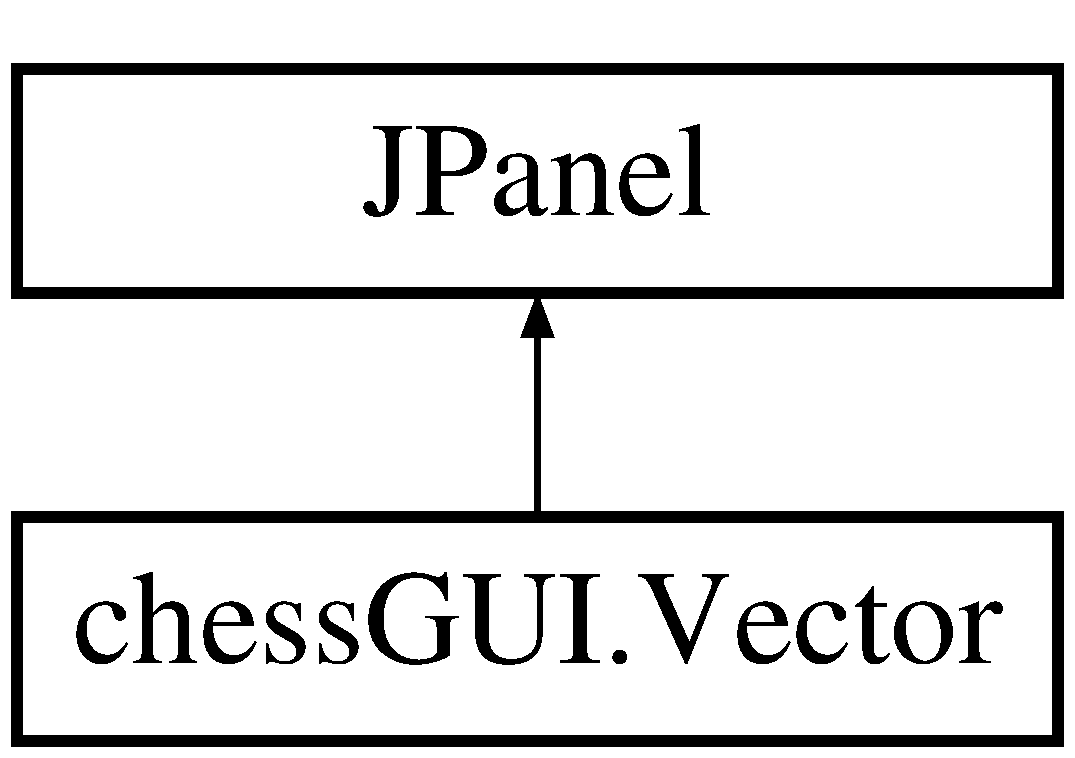
\includegraphics[height=2.000000cm]{classchess_g_u_i_1_1_vector}
\end{center}
\end{figure}


The documentation for this class was generated from the following file\+:\begin{DoxyCompactItemize}
\item 
src/chess\+G\+U\+I/Vector.\+java\end{DoxyCompactItemize}

\hypertarget{classchess_g_u_i_1_1visualize_game}{}\section{chess\+G\+U\+I.\+visualize\+Game Class Reference}
\label{classchess_g_u_i_1_1visualize_game}\index{chess\+G\+U\+I.\+visualize\+Game@{chess\+G\+U\+I.\+visualize\+Game}}
\subsection*{Static Public Member Functions}
\begin{DoxyCompactItemize}
\item 
\mbox{\Hypertarget{classchess_g_u_i_1_1visualize_game_a43d572719c68b08624c43d4178a9b9fa}\label{classchess_g_u_i_1_1visualize_game_a43d572719c68b08624c43d4178a9b9fa}} 
static void {\bfseries main} (String\mbox{[}$\,$\mbox{]} args)
\end{DoxyCompactItemize}


The documentation for this class was generated from the following file\+:\begin{DoxyCompactItemize}
\item 
src/chess\+G\+U\+I/visualize\+Game.\+java\end{DoxyCompactItemize}

%--- End generated contents ---

% Index
\backmatter
\newpage
\phantomsection
\clearemptydoublepage
\addcontentsline{toc}{chapter}{Index}
\printindex

\end{document}
